\documentclass[../main.tex]{subfiles}

\begin{document}
\chapter{Gewöhnliche Differentialgleichungen}\label{chp:odes}
Bevor wir Differentialgleichungen studieren können,
müssen wir den Raum $\mathbb{R}^n$ besser verstehen.
Wir erinnern uns nun an das Studium von Funktionen
in einer Variable.
Dort machen viele Definitionen
vom Absolutbetrag Gebrauch.

\begin{examples}
  \leavevmode
  \begin{enumerate}[(1)]
    \item Konvergenz einer Folge $a \colon \mathbb{N} \to \mathbb{R}$,
      in Symbolen
      \[
        \lim_{n \to \infty} a(n) = \alpha \in \mathbb{R}
      \]
      heisst Folgendes. Für alle $\varepsilon > 0$ existiert
      $N \in \mathbb{N}$, sodass für alle $n \geq N$ 
      gilt, dass $|a(n) - \alpha| \leq \varepsilon$.
    \item Stetigkeit einer Funktion $f \colon \mathbb{R} \to \mathbb{R}$ 
      im Punkt $p\in \mathbb{R}$ heisst, dass für alle $\varepsilon > 0$ 
      ein $\delta > 0$ existiert, so dass
      für alle $q \in \mathbb{R}$ mit $|q - p| \leq \delta$ gilt,
      dass $|f(q) - f(p)| \leq \varepsilon$.
  \end{enumerate}
\end{examples}

Beide dieser sehr zentralen Konzepte machen kritischen Gebrauch
des Absolutbetrags.
In $\mathbb{R}^n$ gibt es aber keinen kanonischen Ersatz für diesen.
Dies motiviert unseren ersten Abschnitt in diesem Kapitel.

\section{Normen auf reellen Vektorräumen}
Die Normaxiome greifen die wichtigsten Eigenschaften des
Absolutbetrags in $\mathbb{R}$ auf und verallgemeinern
diese, so dass wir in allgemeinen reellen Vektorräumen
Konzepte wie Konvergenz und Stetigkeit formalisieren können.

\begin{definition}
  Sei $V$ ein Vektorraum über $\mathbb{R}$.
  Eine Abbildung $\Vert \cdot \Vert \colon V \to \mathbb{R}$
  heisst \emph{Norm} auf $V$, falls folgende Eigenschaften erfüllt werden.
  \begin{enumerate}[(i)]
    \item (Strikte Positivität)
      Für alle $v \in V$ gilt $\Vert v \Vert \geq 0$ und
      $\Vert v \Vert = 0$ genau dann, wenn $v = 0$.
    \item (Homogenität)
      Für alle $v \in V$ und alle $\lambda \in \mathbb{R}$ gilt
      $\Vert \lambda v \Vert = |\lambda| \cdot \Vert v \Vert$.
    \item (Dreiecksungleichung)
      Für alle $v, w \in V$ gilt $\Vert v + w \Vert \leq \Vert v \Vert
      + \Vert w \Vert$.
  \end{enumerate}
\end{definition}

Eigenschaft (ii) hätten wir auch folgendermassen formulieren können:
Die Norm $\Vert \cdot \Vert$ auf einem eindimensionalen Unterraum
von $V$ verhält sich (bis auf Streckung) genau so wie der Absolutbetrag
auf $\mathbb{R}$.

\begin{definition}
  Sei $\Vert \cdot \Vert$ eine Norm auf einem reellen Vektorraum $V$.
  Die Menge
  \[
    B_1 = \left\{v \in V \mid \Vert v \Vert \leq 1\right\} \subset V
  \]
  heisst \emph{Norm-Einheitsball}.
\end{definition}

\begin{examples}
  Sei $V = \mathbb{R}^n$ mit Standardbasis $e_1, \dots, e_n$.
  Einen Vektor $v \in V$ können wir dann ausdrücken durch
  $v = v_1 e_1 + \cdots + v_n e_n$ mit $v_i \in \mathbb{R}$.
  \begin{enumerate}[(1)]
    \item Die \emph{Summennorm} ist die Norm
      \[
        \Vert v \Vert_1 = |v_1| + \cdots + |v_n|.
      \]
      Wir prüfen nun die Normaxiome.
      \begin{enumerate}[(i)]
        \item Dank den Eigenschaften des
          Absolutsbetrag auf $\mathbb{R}$ haben wir sofort 
          $\Vert v \Vert_1 \geq 0$ 
          und $\Vert v \Vert_1 = 0$ genau dann, wenn alle $v_i$ null sind.
        \item Berechne $\Vert \lambda v \Vert_1
          = |\lambda v_1| + \cdots |\lambda v_n| = |\lambda| \cdot
          \Vert v \Vert_1$.
        \item Berechne
          \begin{align*}
            \Vert v + w \Vert_1
            &= |v_1 + w_1| + \cdots + |v_n + w_n| \\
            & \leq |v_1| + |w_1| + \cdots + |v_n| + |w_n| \\
            &= \Vert v \Vert_1 + \Vert w \Vert_1.
          \end{align*}
      \end{enumerate}
    \item Die \emph{Maximumnorm}
      ist die Norm
      \[
        \Vert v \Vert_{\infty}
        = \max \{ |v_1|, \dots |v_n|\}.
      \]
      Wir prüfen wieder die Normaxiome.
      \begin{enumerate}[(i)]
        \item Wir haben $\Vert v \Vert_{\infty} \geq 0$
          und auch $\Vert v \Vert_{\infty}$ genau dann,
          wenn alle $v_i$ null sind.
        \item Es gilt $\Vert \lambda v \Vert_{\infty}
          = \max \left\{\lambda v_1, \dots, \lambda v_n\right\} = |\lambda|
          \cdot \Vert v \Vert_\infty$.
        \item Berechne
          \begin{align*}
            \Vert v + w \Vert_\infty
            &= \max \left\{|v_1 + w_1|, \dots |v_n + w_n|\right\} \\
            &\leq \max \left\{|v_{1}|, \dots, |v_{n}|\right\}
            + \max \left\{|w_{1}|, \dots, |w_{n}|\right\} \\
            &= \Vert v \Vert_{\infty} + \Vert w \Vert_{\infty},
          \end{align*}
          da jeweils $|v_i + w_i| \leq |v_i| + |w_i| $ gilt.
      \end{enumerate}
    \item die \emph{euklidische Norm} ist die Norm
      \[
        \Vert v \Vert_2 = \sqrt{v_1^2 + \cdots v_n^2}.
      \]
      Auch für diese Norm prüfen wir die Axiome.
      \begin{enumerate}[(i)]
        \item Es gilt $\Vert v \Vert_2 \geq 0$ und
          $\Vert v \Vert_2 = 0$ genau dann, wenn
          $v_1^2 + \cdots + v_n^2 = 0$ gilt,
          was äquivalent dazu ist, dass alle $v_i$ null sind.
        \item Berechne $\Vert \lambda v \Vert_2 = |\lambda | \cdot
          \Vert v \Vert_2$, da $\sqrt{\lambda^2} = |\lambda|$ gilt.
        \item Hier stossen wir zum ersten Mal auf Schwierigkeiten.
          Wir werden das im Lemma unten zeigen.
      \end{enumerate}
    \item 
      Folgendes Beispiel rechtfertigt die Notation
      für obige Normen. Sei $p \geq 1$ für $p \geq 1$.
      Die \emph{$p$-Norm} ist
       \[
         \Vert v \Vert_p = \sqrt[p]{|v_1|^p + \cdots + |v_n|^p}.
      \]
      Die Dreiecksungleichung $\Vert v + w \Vert_p \leq
      \Vert v \Vert_p + \Vert w \Vert_p$ heisst
      \emph{Minkowski-Ungleichung}, die aus der
      Konkavität von $\log$ folgt. Siehe hier Abschnitt
      59.3 in~\cite{heuser}.
      Die Normen $\Vert \cdot \Vert_1$ und $\Vert \cdot \Vert_2$ 
      sind Spezialfälle dieser Familie von Normen.
      Für alle $p \geq 1$ gilt, dass $\Vert v \Vert_{\infty}
      \leq \Vert v \Vert_p \leq \sqrt[p]{n} \Vert v \Vert_{\infty}$.
      Im Grenzwert $p \to \infty$ erhalten wir
      \[
        \lim_{p \to \infty} \Vert v \Vert_p = \Vert v \Vert_{\infty}
      \]
      da $\lim_{p \to \infty} \sqrt[p]{n} = 1$.
  \end{enumerate}
  Die Normbälle der ersten drei Normen im Fall $n = 2$
  sind in Abbildung~\ref{fig:norms}
  zu sehen.
\end{examples}

\begin{figure}[htb] 
  \centering
  \begin{minipage}{0.33\textwidth}
    \centering
    \includegraphics{figures/sumnorm}
  \end{minipage}%
  \begin{minipage}{0.33\textwidth}
    \centering
    \includegraphics{figures/maxnorm}
  \end{minipage}%
  \begin{minipage}{0.33\textwidth}
    \centering
    \includegraphics{figures/euclideannorm}
  \end{minipage}%
  \caption{Normbälle der Normen
  $\Vert \cdot \Vert_1,
 \Vert \cdot \Vert_{\infty},
 \Vert \cdot \Vert_2$}%
  \label{fig:norms}
\end{figure}

\subsection*{Normen aus Skalarprodukten}
\begin{definition}
  Ein \emph{Skalarprodukt} auf einem reellen Vektorraum $V$ 
  ist eine strikt positive, symmetrische, bilineare Abbildung
  $\langle \cdot, \cdot \rangle \colon V \times V \to \mathbb{R}$.
  Das heisst,
  \begin{enumerate}[(i)]
    \item für alle $v \in V$ gilt $\langle v, v \rangle \geq 0$ 
      und $\langle v, v \rangle = 0$ genau dann,
      wenn $v = 0$,
    \item für alle $v, w \in V$ gilt 
      $\langle v, w \rangle = \langle w, v \rangle$,
    \item für alle $u, v, w \in V$ und $t \in \mathbb{R}$ gilt
      $\langle u, v + tw \rangle = \langle u, v \rangle + t
      \langle u, w \rangle$.
  \end{enumerate}
\end{definition}

\begin{lemma*}
  Sei $\langle \cdot, \cdot \rangle$ ein Skalarprodukt auf $V$.
  Dann ist die Abbildung
  \begin{align*}
    \Vert \cdot \Vert \colon V & \to \mathbb{R} \\
    v & \mapsto \sqrt{\langle v, v \rangle}
  \end{align*}
  eine Norm auf $V$.
\end{lemma*}

\begin{proof}
  Wir prüfen die Normaxiome folgendermassen.
  \begin{enumerate}[(i)]
    \item Es gilt $\Vert v \Vert = \sqrt{\langle v, v \rangle} \geq 0$
      und $\Vert v \Vert = 0$ genau dann, wenn
      $\langle v, v \rangle = 0$, das heisst, $v = 0$ gilt.
    \item Berechne $\Vert \lambda v \Vert = \sqrt{\langle \lambda v,
      \lambda v\rangle}
      = \sqrt{\lambda^2 \cdot \langle v, v \rangle} = |\lambda| \cdot
      \Vert v \Vert$.
    \item Seien $v, w \in V$. Wir wollen zeigen, dass
      $\sqrt{\langle v + w, v + w \rangle} \leq
      \sqrt{\langle v, v \rangle} + \sqrt{\langle w, w \rangle}$.
      Da Quadrieren auf $\mathbb{R}_{\geq 0}$ monoton ist,
      reicht es zu zeigen, dass
      \[
      \langle v + w, v+ w \rangle\leq \langle v, v \rangle
      + \langle w, w \rangle + 2 \cdot \sqrt{\langle v, v \rangle} \cdot
      \sqrt{\langle w, w \rangle}.
      \]
      Ausmultiplizieren der linken Seite und Subtraktion der Terme,
      die dann auf beiden Seiten erscheinen liefert, dass
      die Dreiecksungleichung für $\Vert \cdot \Vert$ äquivalent
      zur \emph{Cauchy-Schwarz Ungleichung}
      \[
        \langle v, w \rangle \leq \sqrt{\langle v, v \rangle}
        \cdot \sqrt{\langle w, w \rangle}
      \]
      ist.
      Wir beweisen nun diese.
      Betrachte dazu die Funktion $h \colon \mathbb{R} \to \mathbb{R}$,
      die durch
      \[
        h(t) = \langle v + tw, v + tw \rangle \geq 0
      \]
      definiert ist.
      Es gilt also $h(t) = t^2 \langle w, w \rangle + 2t \langle v, w \rangle
      + \langle v, v \rangle$.
      Dies beschreibt eine Parabel mit Diskriminante
      \[
        D = b^2 - 4ac = 4\langle v, w \rangle^2 - 4\langle w, w \rangle
        \cdot \langle v, v \rangle.
      \]
      Aus $h(t) \geq 0$ für alle $t \in \mathbb{R}$ folgt, dass
      $D \leq 0$ ist.
      Wir schliessen, dass $\langle v, w \rangle^2 \leq \langle w, w \rangle
      \cdot \langle v, v \rangle$ gelten muss.
      \qedhere
  \end{enumerate}
\end{proof}

\begin{examples}
  \leavevmode
  \begin{enumerate}[(1)]
    \item Sei $V = \mathbb{R}^n$ und
      \[
        \langle v, w \rangle = v_1 w_1 + \cdots + v_n w_n
      \]
      das \emph{Standardskalarprodukt}.
      Dann ist
      \[
        \Vert v \Vert = \sqrt{v_1^2 + \cdots + v_n^2} = \Vert v \Vert_2
      \]
      die euklidische Norm.
    \item Sei $V = C[0, 1]$ der Raum von stetigen Funktionen
      $f \colon[0, 1] \to \mathbb{R}$.
      Das ist ein unendlichdimensionaler Vektorraum,
      da die Funktionen $1, x, x^2, \dots$ linear unabhängig sind.
      Für $f, g \in V$ definieren wir
      \[
        \langle f, g \rangle = \int_{0}^{1} f(x) \cdot g(x) \, dx.
      \]
      Die Skalarproduktaxiome sind leicht zu überprüfen.
  \end{enumerate}
\end{examples}

\begin{remark}
  Nicht jede Norm auf $V$ stammt von einem Skalarprodukt.
  In den Übungen wird gezeigt, dass jede von einem Skalarprodukt
  induzierte Norm $\Vert \cdot \Vert$ die
  \emph{Parallelogramm-identität}
  \[
    \Vert v + w \Vert^2 + \Vert v - w \Vert^2 
    = 2(\Vert v \Vert^2 + \Vert w \Vert^2)
  \]
  erfüllt, und dass die Normen $\Vert \cdot \Vert_1$ 
  und $\Vert \cdot \Vert_{\infty}$ diese nicht erfüllen.
\end{remark}

\section{Stetigkeit}\label{sec:continuity}
\begin{definition}
  Seien $V$ und $W$ reelle Vektorräume mit Normen $\Vert \cdot \Vert_V$ 
  und
  $ \Vert \cdot \Vert_W$.
  Eine Abbildung $f \colon V \to W$ heisst \emph{stetig
  im Punkt} $p \in V$, falls für alle $\varepsilon > 0$ 
  ein $\delta > 0$ existiert, so dass für alle
  $q \in V$ mit $\Vert q - p \Vert_V \leq \delta$ 
  folgt, dass
  $\Vert f(q) - f(p) \Vert_W \leq \varepsilon$.
  Wir sagen, dass $f$ \emph{stetig} ist, falls
  $f$ in allen Punkten von $V$ stetig ist.
\end{definition}

\begin{example}
  Im Fall $V = W = \mathbb{R}$ und $\Vert \cdot \Vert = \vert \cdot \vert$ 
  erhalten wir den üblichen Stetigkeitsbegriff.
\end{example}

Wir untersuchen nun,
wie der Stetigkeitsbegriff von den Normen
auf  $V$ und $W$ abhängt.
Betrachte zunächst folgenden günstigen Fall.
Sei $V = W = \mathbb{R}$. Sei $\Vert \cdot \Vert$ 
eine Norm auf $\mathbb{R}$.
Für alle $x \in \mathbb{R}$ gilt dann
\[
  \Vert x \Vert = \Vert x \cdot 1 \Vert = |x| \cdot \Vert 1 \Vert.
\]
Sei nun $f \colon \mathbb{R} \to \mathbb{R}$
bezüglich der Norm $| \cdot |$ im Punkt $p \in \mathbb{R}$ stetig.
Wir zeigen nun, dass $f$ auch bezüglich der Norm $\Vert \cdot \Vert$ 
im Punkt $p$ stetig ist.
Wähle $\delta > 0$ so, dass für alle $q \in \mathbb{R}$ 
mit $|q - p| \leq \delta/\Vert 1 \Vert$ gilt,
dass $|f(q)  f(p) \leq \varepsilon/\Vert 1 \Vert$.
Das geht, da $\Vert 1 \Vert > 0$ aus $1 \neq 0$ folgt.
Sei nun $q \in \mathbb{R}$ mit $\Vert q - p \Vert \leq \delta$.
Dann gilt $|q - p| \leq \delta / \Vert 1 \Vert$.
Wir schliessen, dass $|f(q) - f(p)| \leq \varepsilon/\Vert 1 \Vert$,
also 
$\Vert f(q) - f(p) \Vert = |f(q) - f(p)| \cdot \Vert 1 \Vert \leq \varepsilon$.
Insgesamt hängt also der Stetigkeitsbegriff auf $\mathbb{R}$ nicht von
der Norm auf $\mathbb{R}$ ab.

Es gibt aber auch einen ungünstigen Fall.
Sei $\mathbb{R}^{\infty}$ der Raum aller Folgen
$(x_{1}, x_{2}, \dots) \in \mathbb{R}^{\mathbb{N}}$ 
für welche $N > 0$ existiert, so dass für alle $n \geq N$ 
gilt, dass $x_n = 0$.
Betrachte auf $\mathbb{R}^{\infty}$ die beiden Normen
\begin{align*}
  \Vert v \Vert_2 & = \sqrt{v_1^2 + v_2^2 + \cdots} \\
  \Vert v \Vert_{\infty} &= \max \{|v_1|, |v_2|, \dots\}.
\end{align*}
Es gilt für alle $v \in \mathbb{R}^{\infty}$,
dass $\Vert v \Vert_{\infty} \leq \Vert v \Vert_2$.
Sei $V = (\mathbb{R}^{\infty}, \Vert \cdot \Vert_2)$ 
und $W = (\mathbb{R}^{\infty}, \Vert \cdot \Vert_{\infty})$.
Die Identitätsabbildung
\begin{align*}
  \text{Id} \colon \mathbb{R}^{\infty} & \to \mathbb{R}^{\infty} \\
  v & \mapsto v
\end{align*}
kann auf vier Arten als Abbildung zwischen normierten Räumen
betrachtet werden, nämlich
\begin{itemize}
  \item $f_1 \colon V \to V$,
  \item $f_2 \colon W \to W$,
  \item $f_3 \colon V \to W$,
  \item $f_4 \colon W \to V$.
\end{itemize}
Wir bemerken, dass $f_1$, $f_2$ und $f_3$ stetig
sind, indem wir $\delta = \varepsilon$ wählen.
Aber $f_4$ ist nicht stetig!.
Betrachte dazu die Folge von Punkten
$p_n = (1/n, 1/n, \dots, 1/n, 0, \dots) \in \mathbb{R}^{\infty}$,
wobei das Glied $1/n$ gerade $n^2$ mal vorkommt.
Es gilt $\Vert p_n \Vert_{\infty} = 1/n$ 
und $\Vert p_n \Vert_{2} = 1$.
Insbesondere gilt
\[
  \Vert f_4(p_n) - f_4(0) \Vert_2 = \Vert p_n \Vert_2 = 1
\]
und $\Vert p_n \Vert_{\infty} = 1/n$,
also ist $f_4$ im Punkt $p = 0$ nicht stetig.

Zusammengefasst erkennen wir, dass auf $\mathbb{R}^{\infty}$ 
das Verhältnis der Normen $\Vert \cdot \Vert_2$ 
und $\Vert \cdot \Vert_{\infty}$ beliebig hohe Werte annimmt.
Im Sinne folgender Definition bedeutet das, dass in
$\mathbb{R}^{\infty}$ diese beiden normen nicht äquivalent sind.

\begin{definition}
  Zwei Normen $\Vert \cdot \Vert$, $\widetilde{\Vert \cdot \Vert}$
  heissen \emph{äquivalent},
  falls es Konstanten $0 < c \leq C$ gibt,
  so dass für alle $v \in V \setminus \{0\}$ gilt, dass
  \[
    c \leq \frac{\widetilde{\Vert v \Vert}}{\Vert v \Vert} \leq C.
  \]
\end{definition}

Bildlich können wir uns die Äquivalenz von Normen so vorstellen,
dass der $\widetilde{\Vert \cdot \Vert}$-Normball
sowohl eine skalierte Version vom $\Vert \cdot \Vert$-Normball
enthält, wie auch in einer skalierten Version
vom $\Vert \cdot \Vert$-Normball enthalten ist.

\begin{examples}
  \leavevmode
  \begin{enumerate}[(1)]
    \item Sei $\Vert \cdot \Vert$ eine Norm auf $\mathbb{R}$.
      Dann gilt für alle $x \in \mathbb{R}$, dass
      \(
        \Vert x \Vert = \Vert 1 \Vert \cdot |x|,
      \)
      also sind $\Vert \cdot \Vert$ und $| \cdot |$ äquivalent.
    \item
      Für alle $v \in \mathbb{R}^n$ gilt, dass
      \[
        \Vert v \Vert_{\infty} \leq \Vert v \Vert_2
        \leq \sqrt{n} \cdot \Vert v \Vert_{\infty}.
      \]
      also sind die beiden Normen
      $\Vert \cdot \Vert_{\infty}$ und $\Vert \cdot \Vert_2$ 
      äquivalent auf $\mathbb{R}^{n}$.
    \item Auf $\mathbb{R}^{\infty}$ sind die Normen
      $\Vert \cdot \Vert_{\infty}$ und $\Vert \cdot \Vert_{2}$ 
      nicht äquivalent.
  \end{enumerate}
\end{examples}

\begin{remark}
  Die Äquivalenz von Normen ist eine Äquivalenzrelation.
  Die Symmetrie und die Reflexivität sind leicht zu überprüfen.
  Für die Transitivität bemerke, dass
  aus $a \leq x/y \leq A$ und $b \leq y/z \leq B$ folgt,
  dass $ab \leq x/z \leq AB$.
\end{remark}

\begin{theorem*}
  Auf $\mathbb{R}^n$ sind alle Normen äquivalent.
\end{theorem*}

\begin{proof}
  Es reicht zu zeigen, dass jede Norm
  $\Vert \cdot \Vert$ auf $\mathbb{R}^{n}$ 
  zur euklidischen Norm $\Vert \cdot \Vert_2$ 
  äquivalent ist.
  In einem ersten Schritt zeigen wir, dass
  eine Konstante $C > 0$ existiert, so dass
  $\Vert \cdot \Vert / \Vert \cdot \Vert_2 \leq C$
  gilt.
  Sei $v = v_1 e_1 +\cdots + v_n e_n$ mit $v_i \in \mathbb{R}$.
  Schätze ab, dass
  \begin{align*}
    \Vert v \Vert 
    &\leq \Vert v_1 e_1 \Vert + \cdots + \Vert v_n e_n \Vert \\
    &= |v_1| \cdot \Vert e_1 \Vert + \cdots + |v_n| \cdot \Vert e_n \Vert \\
    &\leq \Vert v \Vert_2 \cdot (\Vert e_1 \Vert + \cdots + \Vert e_n \Vert).
  \end{align*}
  Wir erhalten das gewünschte Resultat, indem wir
  $C = \Vert e_1 \Vert + \cdots + \Vert e_n \Vert$ setzen,
  dann gilt nämlich $\Vert v \Vert \leq C \cdot \Vert v \Vert_2$.

  Wir suchen nun im zweiten Schritt
  eine Konstante $c > 0$, für die $\Vert \cdot \Vert / \Vert \cdot \Vert_2
  \geq c$ gilt.
  Nimm widerspruchsweise an, dass das Verhältnis $\Vert \cdot \Vert /
  \Vert \cdot \Vert_2$ beliebig kleine Werte annimmt.
  Dann gibt es eine Folge von Vektoren
  $v_k \in \mathbb{R}^n \setminus \{0\}$ mit
  $\Vert v_k \Vert / \Vert v_k \Vert_2 \leq 1/k$.
  Für die normierten Vektoren $w_k = v_k / \Vert v_k \Vert_2
  \in \mathbb{R}^n \setminus \{0\}$ 
  gilt dann, dass $\Vert w_k \Vert_2 = 1$ 
  und $\Vert w_k \Vert \leq 1/k$.
  Somit liegen alle Koordinaten von $w_k$ 
  im Intervall $[-1, 1]$.
  Also existiert eine Teilfolge
  der $w_k$, so dass die erste Koordinatenfolge
  mit Grenzwert in $[-1, 1]$ konvergiert.
  Wir iterieren dieses Verfahren $n$-mal,
  und erhalten eine Teilfolge $w_{k_i}$ der $w_k$,
  welche in allen Koordinaten konvergiert.
  Setze $w = \lim_{i \to \infty} w_{k_i}$.
  Wir behaupten nun, dass $\Vert w \Vert_2 = 1$ 
  und $\Vert w \Vert = 0$ gilt, was
  natürlich den Widerspruch $w = 0$ impliziert.
  Bemerke dazu, dass für alle $i \in \mathbb{N}$ 
  gilt, dass
  \begin{align*}
     1 - \Vert w - w_{k_i} \Vert_2
     &= \Vert w_{k_i} \Vert_2 - \Vert w - w_{k_i} \Vert_2  \\
     &\leq \Vert w \Vert_2 \\ 
     &\leq \Vert w - w_{k_i} \Vert_2 + \Vert w_{k_i} \Vert_2 \\
    &= 1 + \Vert w - w_{k_i} \Vert_2.
  \end{align*}
  Da die $w_{k_i}$ koordinatenweise gegen $w$ konvergieren, folgt, dass
  \[
    \lim_{i \to \infty} \Vert w - w_{k_i}\Vert_2 = 0
  \]
  gilt. Schätze weiterhin ab, dass
  \[
     \Vert w \Vert
     \leq \Vert w_{k_i} \Vert + \Vert w - w_{k_i} \Vert ,
  \]
  also existiert nach Schritt 1 eine Konstante
  $C > 0$, sodass $\Vert w \Vert \leq 1/k_i + C \cdot
  \Vert w - w_{k_i} \Vert_2$
  gilt, woraus im Grenzwert $i \to \infty$ folgt,
  dass $\Vert w \Vert = 0$ gilt.
\end{proof}

\begin{corollary}\label{cor:continuity-independent}
  Der Stetigkeitsbegriff für Abbildungen
  $f \colon \mathbb{R}^n \to \mathbb{R}^m$ 
  hängt nicht von den Normen auf $\mathbb{R}^n$ 
  und $\mathbb{R}^m$ ab.
\end{corollary}

Der Beweis hier lässt sich durch einfache Ajustierung
der $\delta$ und $\varepsilon$ führen.
Siehe dazu unseren Beweis für den Fakt,
dass alle Normen auf $\mathbb{R}$ zum
selben Stetigkeitsbegriff führen.

\subsection*{Lineare Abbildungen}
\begin{question}
Seien $V, W$ normierte Vektorräume und
$A \colon V \to W$ linear.
Ist $A$ dann stetig?
\end{question}

Die Antwort ist im allgemeinen nein, was unsere
Abbildung $f_4$ oben zeigt. Wir untersuchen
nun noch ein weiteres Beispiel.

\begin{example}
  Sei $V = \mathbb{R}^{\infty}$ mit der
  Maximumsnorm $\Vert \cdot \Vert_{\infty}$.
  Definiere $A \colon \mathbb{R}^{\infty} \to \mathbb{R}^{\infty}$ 
  als die lineare Erweiterung der Abbildung $e_k \mapsto ke_k$.
  Setze  $q_k = e_k/k \in \mathbb{R}^{\infty}$.
  Es gilt, dass
  \(
    \Vert q_k - 0 \Vert_{\infty} = \Vert q_k \Vert_{\infty} = 1/k
  \)
  und $\Vert A(q_k) - A(0) \Vert_{\infty} = \Vert e_k - 0 \Vert_{\infty}
  = 1$. Somit ist $A$ im Nullpunkt (und auch in allen anderen Punkten)
  nicht stetig.
\end{example}

\begin{definition}
  Seien $\Vert \cdot \Vert_V$, $\Vert \cdot \Vert_W$ 
  Normen auf normierten Vektorräumen $V, W$.
  Sei $A \colon V \to W$ linear.
  Die \emph{Operatornorm} von $A$ ist
  \[
    \Vert A \Vert_{\text{op}} = \sup
    \left\{\frac{\Vert Av \Vert_W}{\Vert v \Vert_V} \mid v \in
    V \setminus \{0\}\right\} \in \mathbb{R} \cup \{\infty\}.
  \]
\end{definition}

\begin{examples}
  \leavevmode
  \begin{enumerate}[(1)]
    \item Betrachte die Abbildung
      \begin{align*}
        A \colon \mathbb{R}^{\infty} & \to \mathbb{R}^{\infty} \\
        e_k & \mapsto ke_k
      \end{align*}
      auf $\mathbb{R}^{\infty}$ mit der Norm $\Vert \cdot \Vert_{\infty}$.
      Dann gilt $\Vert A \Vert_{\text{op}} = \infty$.
    \item Sei $A \colon \mathbb{R}^2 \to \mathbb{R}^2$ 
      auf $\mathbb{R}^{2}$ mit der euklidischen Norm
      $\Vert \cdot \Vert_2$ die Abbildung, die durch
      die Matrix
      \[
        A =
        \begin{pmatrix}
          a & b \\ c & d
        \end{pmatrix}
      \]
      gegeben ist.
      Bemerke folgende Eigenschaften.
      \begin{enumerate}[(i)]
        \item $A = 0$ genau dann, wenn $\Vert A \Vert_\text{op} = 0$.
        \item Betrachte
          \[
            A =
            \begin{pmatrix}
              0 & 1 \\ 0 & 0
            \end{pmatrix}.
          \]
          Sei $v = (x, y)$.
          Es gilt dann $Av = (y, 0)$, also gilt
          \[
            \frac{\Vert Av \Vert_2}{\Vert v \Vert_2} = \frac{y}{\sqrt{x^2 + y^2} } \leq 1.
          \]
          Für $x = 0$ erhalten wir $1$ für diesen Quotienten,
          also gilt $\Vert A \Vert_{\text{op}} = 1$.
        \item Betrachte die Matrix
          \[
            A =
            \begin{pmatrix}
              1 & 0 \\ 0 & d
            \end{pmatrix}
          \]
          für $d \geq 1$.
          Um $\Vert A \Vert_{\text{op}}$ zu bestimmen
          reicht es, Vektoren der Form $v = (1, 0)$ 
          und $v = (x, 1)$ zu betrachten.
          Es gilt $A(1, 0) = (1, 0)$,
          also ist $\Vert A \Vert_{\text{op}} \geq 1$. 
          Weiter ist
          $A(x, 1) = (x, d)$.
          Wir schliessen, dass für $v = (x, 1)$ gilt, dass
          \[
            \frac{\Vert Av \Vert_2}{\Vert v \Vert_2}
            = \frac{\sqrt{x^2 + d^2}}{\sqrt{x^2 + 1^2}} \leq d.
          \]
          Aber $d$ wird im Fall $x = 0$ angenommen,
          also folgt $\Vert A \Vert_{\text{op}} = d$.
      \end{enumerate}
  \end{enumerate}
\end{examples}

\begin{proposition}
  Sei $A \colon V \to W$ eine lineare Abbildung zwischen
  normierten Vektorräumen.
  Dann ist $A$ stetig, genau dann, wenn
  $\Vert A \Vert_\text{op} < \infty$ gilt.
\end{proposition}

\begin{proof}
Seien $p \in V$ und $\varepsilon > 0$ 
vorgegeben.
Setze
\[
  \delta = \frac{\varepsilon}{\Vert A \Vert_{\text{op}} + 1}.
\]
Sei nun $q \in V$ mit $\Vert q - p \Vert_V \leq \delta$.
Dann gilt
\begin{align*}
  \Vert A(q) - A(p) \Vert_W
  & = \Vert A(q- p)\Vert_W\\
  &\leq \Vert A \Vert_\text{op} \cdot \Vert q - p \Vert_V \\
  & \leq \Vert A \Vert_{\text{op}} \cdot
  \frac{\varepsilon}{\Vert A \Vert_{\text{op}} + 1} \\
  &\leq \varepsilon.
\end{align*}
Somit ist $A$ stetig im Punkt $p \in V$.
Für die Umkehrung, siehe Serie 2.
\end{proof}
  
\begin{specialcase}
  Sei $A \colon \mathbb{R}^n \to \mathbb{R}^m$ linear.
  Schätze $\Vert A \Vert_{\text{op}}$ bezüglich
  der Maximumsnorm $\Vert \cdot \Vert_{\infty}$ auf
  $\mathbb{R}^n$ und $\mathbb{R}^m$ wie folgt ab.
  Schreibe
  \[
    A = 
    \begin{pmatrix}
      a_{11} & \cdots & a_{1n} \\
      \vdots & \ddots & \vdots \\
      a_{m1} & \cdots & a_{mn}
    \end{pmatrix}
  \]
  als Matrix, das heisst $A(e_i) = \sum_{j=1}^{m} a_{ij}e_j$. 
  Setze $a = \max \left\{|a_{ij}| \mid 
  1 \leq i \leq m, 1 \leq j \leq n\right\}$.
  Für $v \in \mathbb{R}^{n}$ gilt dann
  \(
    \Vert Av \Vert_\infty \leq n \cdot a \cdot \Vert v \Vert_{\infty}.
  \)
  Insbesondere ist $\Vert A \Vert_{\text{op}} \leq n \cdot a$ endlich.
  Wir schliessen, dass $A \colon \mathbb{R}^n \to \mathbb{R}^m$ stetig ist.
\end{specialcase}

\begin{corollary}
  Lineare Abbildungen $A \colon \mathbb{R}^n \to \mathbb{R}^m$ sind stetig.
\end{corollary}

\begin{proof}
  Wir haben soeben gezeigt, dass $A$ bezüglich der Maximumsnorm stetig ist.
  Aus Korollar~\ref{cor:continuity-independent} folgt, dass
  $A$ bezüglich jeder Norm stetig ist.
\end{proof}

\section{Der Fixpunktsatz von Banach}
\begin{motivation}
  Sei $V$ ein normierter reeller Vektorraum,
  und sei $A \colon V \to V$ linear und \emph{kontrahierend},
  das heisst, % A linear schon vorgegeben
  $\Vert A \Vert_{\text{op}} < 1$ gilt.
  Wir wollen die Abbildung $\text{Id} - A \colon V \to V$ wie folgt
  invertieren:
  \[
    {(\text{Id} - A)}^{-1} = \textup{Id} + A + A^2 + A^3 + \cdots
  \]
  Als Analogie dazu erinnern wir uns an den Fakt, dass
  für $q \in \mathbb{R}$ mit $|q| < 1$ gilt, dass
  \[
    \frac{1}{1-q} = 1 + q + q^2 + \cdots.
  \]

  Für alle $Y \in V$ suchen wir ein eindeutiges $X \in V$ 
  mit $(\text{Id} - A)(X) = Y$, also
  $X - A(X) = Y$.
  Definiere
  \begin{align*}
    f \colon V & \to V \\
    X & \mapsto A(X) + Y.
  \end{align*}
  Gesucht ist also eine (offenbar eindeutige) Lösung
  der Fixpunkgleichung $f(X) = X$.
\end{motivation}

\begin{remark}
  Die Bedingung $\Vert A \Vert_{\text{op}} < 1$ ist stärker als die
  Bedingung $\Vert A v \Vert_V < \Vert v \Vert_V$ für alle $v
  \in V \setminus \{0\}$.
  Betrachte dazu $V = \mathbb{R}^{\infty}$ mit der Maximumnorm
  $\Vert \cdot \Vert_{\infty}$.
  Definiere $A \colon \mathbb{R}^{\infty} \to \mathbb{R}^{\infty}$ 
  als die Lineare Erweiterung der Abbildung
  \[
    e_k \mapsto \frac{k}{k+1}e_k.
  \]
  Wir stellen fest, dass $\Vert A v \Vert_{\infty} < \Vert v \Vert_{\infty}$ 
  für alle $v \in \mathbb{R}^{\infty} \setminus \{0\}$ gilt,
  aber $\Vert A \Vert_{\text{op}} = 1$, da
  \[
    \sup \left\{\frac{k}{k+1} \mid k \in \mathbb{N}\right\} = 1
  \]
  gilt. Somit ist $A$ nicht kontrahierend.
  
  Wir stossen auch auf ein Problem beim Invertieren von
  \begin{align*}
    \text{Id} - A \colon \mathbb{R}^{\infty} & \to \mathbb{R}^{\infty} \\
    e_k & \mapsto \left( 1 - \frac{k}{k+1} \right)e_k
    = \frac{1}{k+1}e_k.
  \end{align*}
  Die inverse Abbildung
  \begin{align*}
    {(\text{Id} - A)}^{-1} \colon \mathbb{R}^{\infty} & \to \mathbb{R}^{\infty} \\
    e_k & \mapsto (k+1) e_k
  \end{align*}
  ist also nicht stetig, da $\Vert {(\text{Id} - A)}^{-1} \Vert_{\text{op}}
  = +\infty$.
\end{remark}

\subsection*{Metrische Räume}
\begin{definition}
  Sei $X$ eine Menge. Eine \emph{Metrik} auf $X$ ist eine
  Abbildung $d \colon X \times X \to \mathbb{R}$
  mit folgenden Eigenschaften.
  \begin{enumerate}[(i)]
    \item \emph{Positivität}: Für alle $p, q \in X$ gilt $d(p, q) \geq 0$, und
      $d(p, q) = 0$ genau dann, wenn $p = q$.
    \item \emph{Symmetrie}. Für alle $p, q \in X$ gilt $d(q, p) = d(p, q)$.
    \item \emph{Dreiecksungleichung}. 
      Für alle  $a, b, c \in X$ gilt $d(a, c) \leq d(a, b) + 
      d(b, c)$.
  \end{enumerate}
\end{definition}

\begin{examples}
  \leavevmode
  \begin{enumerate}[(1)]
    \item Sei $V$ ein reeller Vektorraum mit Norm $\Vert \cdot \Vert$.
      Definiere
      \begin{align*}
        d \colon V \times V & \to \mathbb{R} \\
        (p, q) & \mapsto \Vert q - p \Vert.
      \end{align*}
      Das erste Axiom für Metrische Räume folgt direkt aus dem
      ersten Axiom für normierte Räume.
      Zur Symmetrie bemerke, dass
      \[
        d(p, q) = \Vert q - p  \Vert = \Vert (-1)(p - q) \Vert
        = |-1| \cdot \Vert p - q \Vert = \Vert p - q \Vert
        = d(q, p).
      \]
      Die Dreiecksungleichung erfordert keinen Trick.
    \item Sei $X$ beliebig. Definiere auf $X$ 
      die \emph{diskrete Metrik} wie folgt:
      \[
        d (p, q)
        =
        \begin{cases}
          0 & q = p \\
          1 & q \neq p
        \end{cases}.
      \]
      Das einzige interessante Axiom ist die Dreiecksungleichung.
      Falls $d(a, c) = 0$ gilt, dann gilt sowieso
      $d(a, c) \leq d(a, b) + d(b, c)$.
      Der einzige Fall, den wir ausschliessen müssen, ist also
      $d(a, c) = 1$ und $d(a, b) = d(b, c) = 0$.
      Aber aus $d(a, b) = 0$ folgt $a = b$, und
      aus $d(b, c) = 0$ folgt $b = c$ und somit
      auch $a = c$, was $d(a, c) = 0$ impliziert. Dies ist ein
      Widerspruch.
    \item Folgende Metrik ist enorm wichtig in der Zahlentheorie.
      Wir werden sie aber bloss in den Übungen antreffen.
      Sei $p \in \mathbb{N}$ eine Primzahl.
      Definiere die \emph{$p$-adische Metrik} auf $\mathbb{Z}$ 
      wie folgt:
      \[
        d_p(n, m) =
        \begin{cases}
          0 & n = m \\
          p^{-x} & n \neq m,
        \end{cases}
      \]
      wobei $x \in \mathbb{N}$ maximal mit der Eigenschaft
      ist, dass
      $p^x$ die Zahl $n -m $ teilt.
      Insbesondere gilt $d_p(n, n + 1) = 1 = p^{-0}$,
      da in diesem Fall $x = 0$ gilt.
      Weiter ist $d_p(0, p^n) = p^{-n}$, ist also klein für
      grosse $n$.
  \end{enumerate}
\end{examples}

%TODO remove this
\newpage

\begin{definitions}
  Sei $X$ ein metrischer Raum mit Metrik $d$.
  \begin{itemize}
    \item Eine Folge ${(a_{n})}_{n \in \mathbb{N}}$ in
      $X$ heisst \emph{konvergent} mit Grenzwert
      $a \in X$, falls für alle $\varepsilon$ 
      ein $N \in \mathbb{N}$ existiert,
      so dass für alle $n \in \mathbb{N}$ mit $n \geq N$ 
      gilt, dass $d(a_n, a) \leq \varepsilon$.
    \item Eine Folge ${(a_{n})}_{n \in \mathbb{N}}$ in $X$ 
      heisst \emph{Cauchyfolge}, falls für alle $\varepsilon > 0$ 
      ein $N \in \mathbb{N}$ existiert, so dass für
      alle $n, m \geq N$ gilt, dass
      $d(a_n, a_m) \leq \varepsilon$.
    \item Der metrische Raum $X$ heisst \emph{vollständig},
      falls alle Cauchyfolgen in $X$ konvergieren.
  \end{itemize}
  Ein vollständiger normierter Vektorraum heisst \emph{Banachraum}.
\end{definitions}

\begin{examples}
  \leavevmode
  \begin{enumerate}[(1)]
    \item Der metrische Raum $\mathbb{R}$ mit $d(p, q) = |p - q|$ 
      ist vollständig.
    \item
      \begin{enumerate}[(a)]
        \item Der metrische Raum $X = (0, 1) \subset \mathbb{R}$ 
          mit der von $\mathbb{R}$ induzierten
          Metrik $d(p, q) = |q - p|$ ist unvollständig.
        \item Ebenso ist $X = \mathbb{Q} \subset \mathbb{R}$ mit
           der von $\mathbb{R}$ induzierten Metrik unvollständig.
      \end{enumerate}
    \item Sei $X = \mathbb{Z}$ mit der $p$-adischen Metrik $d_p$.
      Betrachte die Folge $a_n = p^n$.
      Dies ist eine Cauchyfolge mit Grenzwert $0 \in \mathbb{Z}$.
      Man könnte nun vermuten, dass $\mathbb{Z}$ mit dieser
      Metrik vollständig ist. Das ist jedoch nicht der Fall.
      Betrachte dazu die Folge $b_n = 1 + p + p^2 + \cdots + p^n$.
      Dies ist eine Cauchyfolge, leider aber ohne Grenzwert
      in $\mathbb{Z}$.
      Das heisst, dass $\mathbb{Z}$ mit der $p$-adischen Metrik
      unvollständig ist. Siehe dazu auch die Übungen.
  \end{enumerate}
\end{examples}

\begin{definition}
  Sei $(X, d)$ ein metrischer Raum.
  Eine Abbildung $f \colon X \to X$ heisst \emph{kontrahierend},
  falls es eine positive Konstante $k < 1$ gibt,
  so dass für alle $p, q \in X$ gilt,
  dass $d(f(p), f(q)) \leq k \cdot d(p, q)$.
\end{definition}

Unser Ziel in diesem Abschnitt ist es,
folgenden wichtigen Satz vom polnischen
Mathematiker Stefan Banach (1892--1945)
zu beweisen.

\begin{theorem*}[Fixpunktsatz von Banach 1922, Heuser 111.11]
  Sei $(X, d)$ ein vollständiger nicht-leerer metrischer Raum.
  Dann hat jede kontrahierende Abbildung
  $f \colon X \to X$ einen eindeutigen Fixpunkt,
  das heisst es existiert genau ein Punkt $p \in X$ 
  mit $f(p) = p$.
\end{theorem*}

\begin{remarks}
  \leavevmode
  \begin{enumerate}[(1)]
    \item Es ist wichtig, dass $k < 1$ gilt.
      Betrachte zum Beispiel folgende Funktionen.
      \begin{enumerate}[(a)]
        \item Betrachte die Abbildung
          \begin{align*}
            f \colon \mathbb{R} & \to \mathbb{R} \\
            x & \mapsto x + 1.
          \end{align*}
          Dann gilt $|f(y) - f(x)| = 1 \cdot |y - x|$,
          aber $f$ hat keinen Fixpunkt.
        \item Die Identität
          \begin{align*}
            f \colon \mathbb{R} & \to \mathbb{R} \\
            x & \mapsto x
          \end{align*}
          hat unendlich viele Fixpunkte.
      \end{enumerate}
    \item Auch die Vollständigkeit ist wichtig.
      Betrachte hier zum Beispiel die Funktion
      \begin{align*}
        f \colon \mathbb{R} \setminus \{0\} & \to \mathbb{R} \setminus \{0\} \\
        x & \mapsto x/2
      \end{align*}
      Die Abbildung $f$ ist kontrahierend mit $k = 1/2$,
      hat aber keinen Fixpunkt in $\mathbb{R} \setminus \{0\}$.
      In den Übungen werden wir ein weniger künstliches Beispiel
      untersuchen.
    \item 
      Kontrahierende Abbildungen $f \colon X \to X$ 
      sind wie alle Lipschitz-stetigen Abbildungen
      $g \colon X \to X$ gleichmässig stetig:
      Sei $L \geq 0$ so, dass für alle
      $p, q \in X$ 
      gilt, dass
      $d(g(p), g(q)) \leq L \cdot d(p, q)$.
      Sei $\varepsilon > 0$ vorgegeben.
      Setze $\delta = \varepsilon/(L+1)$.
      Dann gilt für alle $p, q \in X$ mit $d(p, q) \leq \delta$,
      dass $d(f(p), f(q)) \leq \varepsilon$.
  \end{enumerate}
\end{remarks}

\begin{lemma*}
  Seien $(X_1, d_1)$ und $(X_2, d_2)$ metrische Räume.
  Sei $f \colon X_1 \to X_2$ eine beliebige Abbildung.
  Dann ist $f$ stetig im Punkt $p$, genau dann, wenn $f$ 
  folgenstetig in $p$ ist.
  Folgenstetig heisst, dass für alle konvergenten Folgen
  ${(a_{n})}_{n \in \mathbb{N}}$ in $X_1$ mit
  $\lim_{n \to \infty} a_n = p$ gilt,
  dass $\lim_{n \to \infty} f(a_n) = f(p)$.
\end{lemma*}
 
\begin{proof}
  Für die Richtung ``$\Rightarrow$'',
  sei $f$ stetig in $p$ und ${(a_{n})}_{n \in \mathbb{N}}$
  konvergent mit Grenzwert 
  $\lim_{n \to \infty} a_n = p$.
  Sei $\varepsilon > 0$ vorgegeben.
  Wähle $\delta > 0$ so, dass wenn
  $d_1(q, p) \leq \delta$ gilt,
  dann auch $d_2(f(q), f(p)) \leq \varepsilon$.
  Dann existiert $N \in \mathbb{N}$ so,
  dass für $n \geq N$ gilt, dass
  $d(a_n, p) \leq \delta$.
  Somit gilt auch für alle $n \geq N$,
  dass $d_2(f(a_n), f(p)) \leq \varepsilon$.
  Somit ist $f$ folgenstetig.

  Umgekehrt, für ``$\Leftarrow$'',
  sei $f$ nicht stetig in $p$.
  Dann existiert $\varepsilon > 0$ so,
  dass für alle $n \in \mathbb{N}$ ein
  $a_n \in X_1$ existiert mit
  $d_1(a_n, p) \leq 1/n$, aber
  $d_2(f(a_n), f(p)) > \varepsilon$.
  Nach Konstruktion gilt
  $\lim_{n \to \infty}a_n = p$,
  aber $\lim_{n \to \infty}f(a_n) \neq f(p)$.
  Folglich ist $f$ nicht folgenstetig in $p$.
\end{proof}

\begin{proof}[Beweis vom Fixpunktsatz]
  Wir zeigen erst die Eindeutigkeit,
  was ganz schnell geht.
  Seien $p, q \in X$ Fixpunkte von $f$.
  Dann gilt $d(f(p), f(q)) \leq k \cdot d(p, q)$.
  Aus $k < 1$ folgt dann $d(p, q) = 0$,
  also $q = p$.

  Für die Existenz, wähle $a_0 \in X$. Dieser
  Schritt ist der Grund für die Annahme,
  dass $X$ nicht leer ist.
  Definiere eine Folge in $X$ durch die
  Vorschrift $a_{n+1}= f(a_n)$.
  Es gilt dann $a_1 = f(a_0), a_2 = f^2(a_0) = f(f(a_0))$,
  und allgemein $a_n = f^n(a_0)$.
  Die so konstruierte Folge ${(a_{n})}_{n \in \mathbb{N}}$ 
  ist eine Cauchyfolge in $X$. Wir zeigen das später
  und nehmen vorerst an, dass das stimmt.
  Da $X$ vollständig ist, existiert $X \ni p = \lim_{n \to \infty} a_n$.
  Es gilt dann $f(p) = p$.
  Tatsächlich, berechne
  \[
  f(p) = \lim_{n \to \infty} f(a_n) = \lim_{n \to \infty}a_{n+1} = p.
  \]
  Es bleibt also bloss zu zeigen,
  dass $ {(a_n)}_{n \in \mathbb{N}}$
  eine Cauchyfolge ist.
  Sei dazu $\varepsilon > 0$ vorgegeben.
  Für $n, m \in \mathbb{N}$ mit $n \geq m$ 
  schätzen wir ab, dass
  \begin{align*}
    d(a_n, a_m)
    & = d(f(a_{n-1}), f(a_{m-1}))\\
    & \leq k \cdot d(a_{n-1}, a_{m-1}) \\
    &\leq k^2 \cdot d(a_{n-2}, a_{m-2})\\
    &\leq \cdots \\
    &\leq k^m \cdot d(a_{n-m}, a_0).
  \end{align*}
  Setze $\ell = n -m $.
  Schätze weiterhin ab, dass
  \begin{align*}
    d(a_{\ell}, a_0) 
    &\leq d(a_\ell, a_{\ell - 1})
    + d(a_{\ell - 1}, a_{\ell-2}) + \cdots + d(a_1, a_0)\\
    &\leq k^{\ell-1} \cdot d(a_{1}, a_{0})
    + k^{\ell - 2} \cdot d(a_1, a_0)
    + \cdots
    + d(a_1, a_0) \\
    = (1 + k + k^2 + \cdots + k^{\ell-1})
    \cdot d(a_1, a_0) \\
    &\leq \frac{1}{1-k} \cdot d(a_1, a_0).
  \end{align*}
  Insgesamt erhalten wir
  \[
    d(a_n, a_m) \leq k^m \cdot \frac{1}{1-k} \cdot d(a_1, a_0).
  \]
  Wähle $N \in \mathbb{N}$ so,
  dass $k^N \cdot 1/(1-k) \cdot d(a_1, a_0) \leq \varepsilon$.
  Solch ein $N$ existiert, da 
  nach unseren Annahmen an $k$ gilt,
  dass $\lim_{n \to \infty} k^n = 0$.
  Es gilt dann für alle $n, m \geq N$, dass
  $d(a_n, a_m) \leq \varepsilon$.
\end{proof}

Wir werden den Fixpunktsatz auf Banachräume
anwenden um Sätze zur Existenz und Eindeutigkeit
gewisser Differentialgleichungen zu zeigen.

\begin{example}
  Sei $K \subset \mathbb{R}$ kompakt,
  das heisst $K$ ist beschränkt und abgeschlossen.
  Definiere $C(K)$ als die Menge aller stetigen
  Abbildungen  $f \colon K \to \mathbb{R}$.
  Man kann sich leicht überlegen,
  dass $C(K)$ ein reeller Vektorraum ist.
  Wir statten $C(K)$ mit der Norm
  \[
    \Vert f \Vert_{\infty} =
    \max \left\{|f(x)| \mid x \in K\right\} < +\infty
  \]
  aus. Der Satz von Weierstrass besagt,
  dass für eine Folge $f_n \colon K \to \mathbb{R}$ 
  stetiger Funktionen, welche auf $K$ 
  gleichmässig gegen eine Funktion $f \colon K \to \mathbb{R}$
  konvergiert, $f$ stetig ist.
  Gleichmässige Konvergenz heisst,
  dass für alle $\varepsilon > 0$ 
  ein $N \in \mathbb{N}$ existiert, so dass
  für alle $n \geq N$ und alle $p \in K$ gilt,
  dass $|f_n(p) - f(p)| \leq \varepsilon$.
  In unseren Worten heisst das
  $\Vert f_n - f \Vert_{\infty} \leq \varepsilon$.
  Der Satz von Weierstrass besagt also,
  dass der Raum $C(K)$ mit der Maximumnorm vollständig ist.
\end{example}

\section{Kurven und Vektorfelder}
\begin{definition}
  Eine \emph{Kurve} in $\mathbb{R}^n$ 
  ist das Bild einer stetigen Abbildung
  $\gamma \colon \mathbb{R} \to \mathbb{R}^n$.
  Die Abbildung $\gamma$ heisst
  \emph{Parametrisierung} der Kurve $\gamma$.
  Wir werden die Unterscheidung zwischen Kurven
  und Parametrisierungen nicht immer explizit
  machen.
\end{definition}

Wir untersuchen nun kurz den Stetigkeitsbegriff auf Kurven.
Stetigkeit heisst, dass in jedem $t \in \mathbb{R}$ die
$(\varepsilon, \delta)$-Bedingung für $\gamma$ 
bezüglich beliebiger Normen auf $\mathbb{R}$ und $\mathbb{R}^n$ 
erfüllt ist, insbesondere
bezüglich der Normen $| \cdot |$ und $\Vert \cdot \Vert_{\infty}$.
Schreibe nun 
\[
  \gamma(t) = \sum_{i=1}^{n} \gamma_i(t) \cdot e_i,
\]
wobei $e_i$ der $i$-te Basisvektor in $\mathbb{R}^n$ ist.
In diesem Fall ist $\gamma_i(t) = \langle \gamma(t), e_i \rangle$  % für Standardskalarprodukt; nicht für SkP allgemein, oder?
die $i$-te Komponentenfunktion von $\gamma$.
Für alle $s, t \in \mathbb{R}$ gilt
$\Vert \gamma(s) - \gamma(t) \Vert_\infty \leq \varepsilon$ 
genau dann, wenn $|\gamma_i(s) - \gamma_i(t)| \leq \varepsilon$
für alle  $i$.
Wir folgern, dass $\gamma$ stetig in $t \in \mathbb{R}$ 
ist, genau dann wenn alle Komponentenfunktionen
$\gamma_i$ stetig in $t$ sind.

\begin{example}
  \leavevmode
  \begin{enumerate}[(1)]
    \item 
      Betrachte die Funktion
      \begin{align*}
        \gamma \colon \mathbb{R} & \to \mathbb{R}^2 \\
        t & \mapsto (\cos(t), \sin(t)).
      \end{align*}
      Dann hat $\gamma$ stetige
      Komponentenfunktionen und ist sie
      daher die Parametrisierung einer Kurve.
      In diesem Fall ist die beschriebene Kurve
      der Einheitskreis, siehe Abbildung~\ref{fig:parametrisations}.
      Die Pfeile erklären wir später.
    \item Die Funktion
      \begin{align*}
        \gamma \colon \mathbb{R} & \to \mathbb{R}^2 \\
        t & \mapsto (t^2, t^3 - t)
      \end{align*}
      ist stetig und somit die Parametrisierung einer Kurve,
      dargestellt in Abbildung~\ref{fig:parametrisations}.
      Diese Kurve einen ``singulären Punkt'',
      herbeigeführt durch die Eigenschaft,
      dass $\gamma(1) = \gamma(-1) = 1$ gilt.
  \end{enumerate}
\end{example}

\begin{figure}[htb] 
  \centering
  \begin{minipage}{0.50\textwidth}
    \centering
    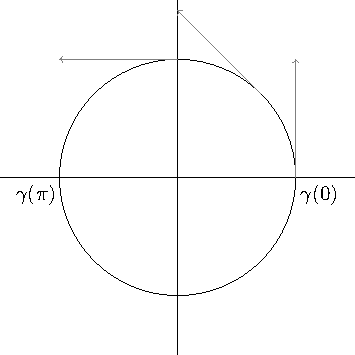
\includegraphics{figures/circlecurve}
  \end{minipage}%
  \begin{minipage}{0.50\textwidth}
    \centering
    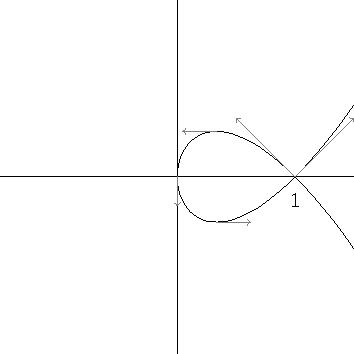
\includegraphics{figures/butterflycurve}
  \end{minipage}%
  \caption{Die Bilder der Kurven $\gamma$ 
  aus den Beispielen}%
  \label{fig:parametrisations}
\end{figure}

\begin{definition}
  Eine parametrisierte Kurve $\gamma \colon \mathbb{R} \to \mathbb{R}^n$ 
  heisst \emph{differenzierbar}, falls für alle $t \in \mathbb{R}$ 
  die Ableitung
  \[
    \dot{\gamma}(t) = \lim_{h \to 0} \frac{ \gamma(t + h) - \gamma(t)}{h}
  \]
  existiert.
  Der Vektor $\dot{\gamma}(t)$ heisst \emph{Geschwindigkeitsvektor}.
\end{definition}

\begin{remark}
  Für alle $t, h \in \mathbb{R}$ mit $h \neq 0$ 
  gilt
  \[
    \frac{\gamma(t + h) - \gamma(t)}{h}
    = \sum_{k=1}^{n} \frac{\gamma_k(t + h)- \gamma_k(t)}{h} \cdot e_k
  \]
  Wir folgern, dass $\dot{\gamma}(t) \in \mathbb{R}^n$ existiert,
  genau dann, wenn alle Ableitungen $\dot{\gamma}_k(t) \in \mathbb{R}$ 
  existieren.
  In anderen Worten: Eine Kurve $\gamma \colon \mathbb{R} \to \mathbb{R}^n$ 
  ist differenzierbar, genau dann, wenn alle $\gamma_k \colon \mathbb{R}
  \to \mathbb{R}$ differenzierbar sind.
\end{remark}

\begin{examples}
  \leavevmode
  \begin{enumerate}[(1)]
    \item Die Kurve
      \begin{align*}
        \gamma \colon \mathbb{R} & \to \mathbb{R}^2 \\
        t & \mapsto (\cos(t), \sin(t))
      \end{align*}
      ist differenzierbar mit $\dot{\gamma}(t) = (-\sin(t), \cos(t))$.
      Die grauen Pfeile in Abbildung~\ref{fig:parametrisations}
      stellen die Ableitung von $\gamma$ dar.
    \item Die Kurve
      \begin{align*}
        \gamma \colon \mathbb{R} & \to \mathbb{R}^2 \\
        t & \mapsto (t^2, t^3 - t)
      \end{align*}
      ist differenzierbar mit $\dot{\gamma}(t) = (2t, 3t^2 - 1)$.
      Wir berechnen
      \begin{itemize}
        \item $\gamma(0) = (0, 0)$ und $\dot{\gamma}(0) = (0, -1)$,
        \item $\gamma(1) = (1, 0)$ und $\dot{\gamma}(1) = (2, 2)$,
        \item $\gamma(-1) = (1, 0)$ und $\dot{\gamma}(-1) = (-2, 2)$,
        \item $\gamma(1/\sqrt{3}) = (1/2, -2/3 \cdot 1/\sqrt{3})$
          und $\dot \gamma (1/\sqrt{3}) = (2 / \sqrt 3, 0)$,
        \item $\gamma(-1 / \sqrt 3) = (1 / 3, 2/ 3 \cdot 1 / \sqrt 3)$
          und $\dot \gamma ( - 1 / \sqrt 3 ) = (- 2 / \sqrt 3, 0)$.
      \end{itemize}
     Für grosse $t$ ist $y$ ungefähr $x^{3/2}$. Diese Information reicht,
     um das Bild von $\gamma$ wie in Abbildung~\ref{fig:parametrisations}
     zu erraten.
     Die Ableitungen sind in grau (mit $1/4$ gestreckt) eingezeichnet.
  \end{enumerate}
\end{examples}

\begin{definition}
  Sei $U \subset \mathbb{R}^n$ offen.
  Ein \emph{Vektorfeld} auf $U$ ist eine stetige Abbildung
  \begin{align*}
    X \colon U & \to \mathbb{R}^n \\
    q & \mapsto X(q).
  \end{align*}
  Jedes Vektorfeld $X$ auf $U$ liefert eine
  \emph{gewöhnliche Differentialgleichung}
  $\dot \gamma(t) = X(\gamma(t))$.
  Dies ist wie folgt zu interpretieren.
  Sei $p \in U$ fest. Gesucht ist $T > 0$ 
  und eine differenzierbare  \emph{Lösungskurve}
  $\gamma  \colon (-T, T) \to U$ 
  zur Anfangsbedingung $\gamma(0) = p$.
  Falls $X = A \colon \mathbb{R}^n \to \mathbb{R}^n$ 
  linear ist, dann heisst die Differentialgleichung
  $\dot \gamma(t) = A(\gamma(t))$
  \emph{linear}.
\end{definition}

\begin{geometric}
  Ein Vektorfeld $X \colon U \to \mathbb{R}^2$ 
  liefert in jedem Punkt $q \in U$ einen Vektor
  $X(q) \in \mathbb{R}^n$.
  Siehe Abbildung~\ref{fig:vectorfield}.
  In jedem Punkt der Kurve
  $\gamma(t) \in U$ stimmt der Geschwindigkeitsvektor
  $\dot \gamma(t) \in \mathbb{R}^n$ 
  mit dem Vektor $X(\gamma(t))$ überein.
\end{geometric}

\begin{figure}[ht]
    \centering
    \incfig{vectorfield}
    \caption{Ein Vektorfeld $X$ auf $U \subset \mathbb{R}^2$
    mit einer Lösungskurve $\gamma$ in schwarz}%
    \label{fig:vectorfield}
\end{figure}

\newpage

\begin{examples}
  \leavevmode
  \begin{enumerate}[(1)]
    \item Betrachte das lineare Vektorfeld
      \begin{align*}
        X \colon \mathbb{R} & \to \mathbb{R}^n \\
        q & \mapsto 0.
      \end{align*}
      Sei $p \in \mathbb{R}^n$. Dann ist $\gamma(t) = p$ 
      die eindeutige
      Lösung der Differentialgleichung $\gamma(0) = p$ 
      und $\dot \gamma(t) = X(\gamma(t))$.
    \item Betrachte das lineare Vektorfeld
      \begin{align*}
        A \colon \mathbb{R}^2 & \to \mathbb{R}^2 \\
        \begin{pmatrix}
          x \\ y
        \end{pmatrix}
         & \mapsto 
         \begin{pmatrix}
           0 & -1 \\ 1 & 0
         \end{pmatrix}
         \begin{pmatrix}
           x \\ y
         \end{pmatrix}
         =
         \begin{pmatrix}
           -y \\ x
         \end{pmatrix},
      \end{align*}
      siehe Abbildung~\ref{fig:vectorfields-examples}.
      Betrachte nochmals die Kurve
      \begin{align*}
        \gamma \colon \mathbb{R} & \to \mathbb{R}^2 \\
        t & \mapsto 
        \begin{pmatrix}
          \cos(t) \\ \sin(t)
        \end{pmatrix}.
      \end{align*}
      Es gilt
      \[
        \dot \gamma(t) =
        \begin{pmatrix}
          - \sin(t) \\ \cos(t)
        \end{pmatrix}
        =
        \begin{pmatrix}
          0 & -1 \\ 1 & 0
        \end{pmatrix}
        \begin{pmatrix}
          \cos(t) \\ \sin(t)
        \end{pmatrix}
        = A(\gamma(t)).
      \]
      Also ist die Kurve $\gamma \colon \mathbb{R} \to \mathbb{R}^2$ 
      eine Lösung der linearen Differentialgleichung
      $\dot \gamma(t) = A(\gamma(t))$ 
      zur Anfangsbedingung $\gamma(0) = e_1 \in \mathbb{R}^2$.
      Allgemeiner ist die Funktion
      \begin{align*}
        \gamma \colon \mathbb{R} & \to \mathbb{R}^2 \\
        t & \mapsto 
        \begin{pmatrix}
          r \cos(t + \varphi) \\
          r \sin(t + \varphi)
        \end{pmatrix}
      \end{align*}
      eine Lösung dieser Differentialgleichung.
      Durch geschickte Wahl von $\varphi$ und $r$
      deckt das jede Anfangsbedingung ab.
      \begin{figure}[htb] 
        \centering
        \begin{minipage}{0.50\textwidth}
          \centering
          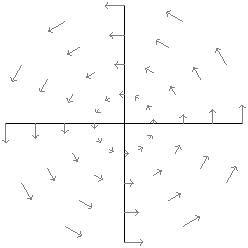
\includegraphics{figures/rotationfield}
        \end{minipage}%
        \begin{minipage}{0.50\textwidth}
          \centering
          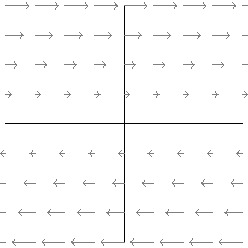
\includegraphics{figures/yzero}
        \end{minipage}%
        \caption{Das Vektorfeld $A(x, y) = (-y, x)$ und das
        Vektorfeld $A(x, y) = (y, 0)$}% ev. noch auf die Bspl. (2 bzw. 4) verweisen :)
        \label{fig:vectorfields-examples}
      \end{figure}
    \item Die Kurve $\gamma(t) = (t^2, t^3 - t)$ ist
      nicht die Lösung einer gewöhnlichen Differentialgleichung.
      Der Grund dafür ist, dass $\gamma$ den Punkt
      $(1, 0)$ zweimal mit unterschiedlichen Geschwindigkeitsvektoren
      durchläuft: Es gilt $\gamma(1) = \gamma(-1)$.
      aber $\dot \gamma(1) \neq \dot \gamma(-1)$.
      Falls nämlich $X \colon \mathbb{R}^2 \to \mathbb{R}^2$ 
      existiert mit $\dot \gamma (t) = X ( \gamma(t))$,
      dann gälte
      \begin{align*}
        X(e_1) &= X(\gamma(1)) = \dot \gamma(1) = (2, 2),\\
        X(e_1) &= X(\gamma(-1)) = \dot \gamma(-1) = (-2, 2).
      \end{align*}
      Das ist aber nicht möglich, da $2 \neq -2$.
    \item Betrachte das lineare Vektorfeld
      \begin{align*}
        A \colon \mathbb{R}^2 & \to \mathbb{R}^2 \\
        \begin{pmatrix}
          x \\ y
        \end{pmatrix}
         & \mapsto 
         \begin{pmatrix}
           0 & 1 \\ 0 & 0
         \end{pmatrix}
         \begin{pmatrix}
           x \\ y
         \end{pmatrix}
         =
         \begin{pmatrix}
           y \\ 0
         \end{pmatrix}.
      \end{align*}
      Sei $p = (x_0, y_0)$ vorgegeben.
      Als Ansatz für $\gamma$
      schreiben wir $\gamma(t) = (x(t),
      y(t))$.
      Aus $\dot \gamma(t) = (y(t), 0)$ erhalten wir
      $\dot y (t) = 0$, also ist $y(t) = y_0$ konstant.
      Weiterhin ist
      $\dot x(t) = y(t) = y_0$, also ist
      $x(t) = y_0 t + x_0$. Zusammengefasst erhalten
      wir die Lösungskurve
      \[
        \gamma(t) =
        \begin{pmatrix}
          x_0 + y_0 t \\
          y_0
        \end{pmatrix}.
      \]
    \item Sei $A \colon \mathbb{R}^n \to \mathbb{R}^n$ 
      beliebig und linear.
      Sei $v \in \mathbb{R}^n$ ein Eigenvektor zum Eigenwert
      $\lambda \in \mathbb{R}$, das heisst
      $A(v) = \lambda v$.
      Definiere
       \begin{align*}
        \gamma \colon \mathbb{R} & \to \mathbb{R}^n \\
        t & \mapsto e^{\lambda t} \cdot v.
      \end{align*}
      Es gilt $\gamma(0) = v$ und
      \[
        \dot \gamma(t) = e^{\lambda t} \cdot \lambda \cdot v
        = e^{\lambda t}  \cdot A(v)
        = A(e^{\lambda t} \cdot v).
      \]
      Also ist $\gamma$ eine Lösungskurve.
      Wir haben aber verwendet, dass $v$ ein Eigenvektor
      von $A$ ist. Die anderen Lösungskurven von $A$ 
      könnten komplizierter sein.
    \item Sei $A \colon \mathbb{R}^n \to \mathbb{R}^n$ 
      linear und \emph{diagonalisierbar} über $\mathbb{R}$,
      das heisst es existieren
      \emph{Eigenwerte} $\lambda_1, \dots, \lambda_n \in \mathbb{R}$ 
      und eine Basis aus \emph{Eigenvektoren}
      $\{v_1, \dots, v_n\}$ von $\mathbb{R}^n$ 
      mit $A(v_i) = \lambda_i v_i$.
      Sei $p \in \mathbb{R}^n$ vorgegeben. Schreibe
      \[
        p = \sum_{i=1}^{n} x_i v_i
      \]
      mit $x_i \in \mathbb{R}$.
      Definiere
      \begin{align*}
        \gamma \colon \mathbb{R} & \to \mathbb{R}^n \\
        t & \mapsto e^{\lambda_1 t} \cdot x_1 \cdot v_1 +
        \cdots
        +
        e^{\lambda_n t} \cdot x_n \cdot v_n.
      \end{align*}
      Es gilt $\gamma(0) = p$ und
      \[
        \dot \gamma(t) = \sum_{i=1}^{n} \lambda_i e^{\lambda_i t}x_i v_i
        = A(\gamma(t)).
      \]
      Es existiert also eine Lösungskurve $\gamma(t)$ 
      für beliebige Anfangsbedingungen.
    \item Sei
      \begin{align*}
        f \colon \mathbb{R} & \to \mathbb{R} \\
        x & \mapsto 2 \sqrt{|x|}
      \end{align*}
      ein Vektorfeld auf $\mathbb{R}$.
      Betrachte die Anfangsbedingung $p = 0$.
      Die konstante Nullkurve ist
      eine Lösungskurve.
      Betrachte nun die Kurve
      \begin{align*}
        \gamma \colon \mathbb{R} & \to \mathbb{R} \\
        t & \mapsto 
        \begin{cases}
          0 & t \leq 0 \\
          t^2 & t \geq 0.
        \end{cases}
      \end{align*}
      Es gilt $\gamma(0) = 0$ und
      \[
        \dot \gamma(t) =
        \begin{cases}
          0 & t \leq 0 \\
          2t & t \geq 0.
        \end{cases}
      \]
      Es gilt aber auch
      \[
        f(\gamma(t)) =
        \begin{cases}
          2 \sqrt{|0|} = 0 & t \leq 0 \\
          2 \sqrt{|t^2|} = 2t & t \geq 0.
        \end{cases}
      \]
      Das heisst $\gamma(t)$ ist auch eine Lösung
      zur selben Anfangsbedingung.
      Das ``Problem'' hier ist,
      dass $f \colon \mathbb{R} \to \mathbb{R}$ 
      nicht Lipschitz-stetig ist.
  \end{enumerate}
\end{examples}

\section{Der Satz von Cauchy-Lipschitz-Picard-Lindelöf}
\begin{definition}
  Sei $U \subset \mathbb{R}^n$ offen.
  Eine Abbildung $X \colon U \to \mathbb{R}^n$ 
  heisst \emph{Lipschitz-stetig} mit Konstante
  $k \geq 0$, falls für alle $p, q \in U$ 
  die Ungleichung
  \[
    \Vert X(q) - X(p) \Vert_2 \leq k \cdot \Vert q - p \Vert_2
  \]
  gilt.
\end{definition}

\begin{remark}
  Die Wahl der Norm $\Vert \cdot \Vert_2$ ist für diese
  Definition irrelevant,
  da alle Normen auf $\mathbb{R}^n$ äquivalent sind.
  Die Konstante $k \geq 0$ hängt aber von der gewählten
  Norm ab.
\end{remark}

\begin{theorem*}[Cauchy-Lipschitz-Picard-Lindelöf]
  Sei $U \subset \mathbb{R}^n$ offen
  und $X \colon U \to \mathbb{R}^n$ Lipschitz-stetig
  mit Konstante $k \geq 0$.
  Sei $p \in U$ vorgegeben.
  Dann existiert $T > 0$ und eine \emph{eindeutige}
  differenzierbare Kurve
  $\gamma \colon (-T, T) \to U$ mit $\gamma(0) = p$,
  so dass für alle $t \in (-T, T)$ gilt, dass
  $\dot \gamma(t) = X(\gamma(t))$.
\end{theorem*}

\begin{remark}
  \leavevmode
  \begin{enumerate}[\normalfont1.]
    \item Falls $U = \mathbb{R}^n$ ist, kann $T > 0$ 
      beliebig gewählt werden.
      Siehe dazu Übungsserie 4.
    \item Falls $U = \mathbb{R}^n$ und $k = 0$, 
      dann gilt für alle $p,q \in \mathbb{R}^n$,
      dass 
      $\Vert X(p)  - X(q) \Vert_2 
      \leq 0 \cdot \Vert p - q \Vert_2 = 0$.
      Das Vektorfeld $X$ ist also konstant.
      Dann ist die Lösungskurve
      \begin{align*}
        \gamma \colon \mathbb{R} & \to \mathbb{R}^n \\
        t & \mapsto p + t \cdot X(p).
      \end{align*}
  \end{enumerate}
\end{remark}


Vergleiche~\cite{heuser}, Satz 117.1.
Ein wichtiger Unterschied in der Version,
die Heuser formuliert, ist es,
dass das Vektorfeld $f$ dort auch von der Zeit $x$
abhängen darf.
Wir werden nun einige Vorbereitungen zum Beweis
treffen.
Dazu werden wir zunächst Kurven genauer betrachten.

\begin{definition}
  Sei $\alpha \colon [a, b] \to \mathbb{R}^n$ stetig.
  Schreibe 
  \[\alpha(t) = \sum_{i=1}^{n} \alpha_i(t) e_i,
  \]
  wobei $\alpha_i \colon [a, b] \to \mathbb{R}$ stetige Funktionen sind.
  Wir schreiben dann
  \[
    \int_{a}^{b} \alpha(s) \, ds
    = \sum_{i=1}^{n} \left( 
      \int_a^b
      \alpha_i(s) \, ds
    \right) \cdot e_i.
  \]
\end{definition}

\begin{proposition}
  Seien $\alpha \colon [a, b] \to \mathbb{R}$ stetig
  und $\gamma \colon (a, b) \to \mathbb{R}$ 
  stetig differenzierbar.
  Dann gilt:
  \begin{enumerate}[\normalfont(i)]
    \item für alle $t \in (a, b)$ gilt
      \[
        \frac{d}{dt} \int_{a}^{t} \alpha(s) \, ds = \alpha(t),
      \]
    \item unter der Annahme, dass $[0, t] \subset (a, b)$, gilt
      \[
        \gamma(t) - \gamma(0) = \int_{0}^{t} \dot \gamma(s) \, ds.
      \]
  \end{enumerate}
\end{proposition}

\begin{proof}
  Sowohl die Differentiation als auch die Integration von Kurven
  lässt sich komponentenweise ausführen.
  Deshalb folgen die beiden Eigenschaften aus den entsprechenden
  Sätzen der Differential- und Integralrechnung für Funktionen
  auf $\mathbb{R}$.
\end{proof}

Sei $C([a, b], \mathbb{R}^n)$ der Raum aller stetiger
Funktionen $\alpha \colon [a, b] \to \mathbb{R}^n$.
Für eine Funktion $\alpha \in C([a, b], \mathbb{R}^n)$ definieren wir
\[
  \Vert \alpha \Vert_{\infty}
  = \max \left\{\Vert \alpha(t) \Vert_2 \mid 
  t \in [a, b]\right\} \geq 0.
\]

\begin{lemma}
  Der Raum $C([a, b], \mathbb{R}^n)$ ist bezüglich der Norm
  $\Vert \cdot \Vert_{\infty}$ vollständig.
\end{lemma}

\begin{proof}
  Sei ${(\alpha_{m})}_{m \in \mathbb{N}}$ 
  eine Cauchyfolge in $V$ bezüglich der Norm % V noch nicht definiert
  $\Vert \cdot \Vert_{\infty}$.
  Dann erhalten wir in jeder Komponente $i \leq n$ 
  eine Cauchyfolge $\langle \alpha_m, e_i \rangle$ 
  in $C([a, b], \mathbb{R})$ (bezüglich der Norm
  $\Vert \cdot \Vert_{\infty}$).
  Nach Weierstrass existiert für alle $i \leq n$ 
  der Grenzwert
  $\lim_{m \to \infty} \langle \alpha_m, e_i \rangle$ 
  in $C([a, b], \mathbb{R})$.
  Es folgt
  wie im Beweis von Banachs Fixpunktsatz, dass der Grenzwert
  \[
    \lim_{m \to \infty} \alpha_m
    = \sum_{i=1}^{n} \lim_{m \to \infty}
    \langle \alpha_m, e_i \rangle \cdot e_i 
  \]
  in $C([a, b], \mathbb{R}^n)$ existiert.
  Also ist $V$ mit der Norm $\Vert \cdot \Vert_\infty$ vollständig.
\end{proof}

% Die Beweisidee vom Theorem ist nun folgendermassen.
% Sei $\gamma \colon (-T, T) \to U$ 
% differenzierbar mit $\gamma(0) = p$ 
% und $\dot \gamma(t) = X(\gamma(t))$.
% Dann ist $\dot \gamma \colon (-T, T) \to \mathbb{R}^n$ 
% stetig, da $X$ stetig ist, und somit auch $X \circ \gamma$.
% Aus Punkt (ii) der Proposition folgt für alle
% $t \in (-T, T)$, dass
% \[
%   \gamma(t) - \gamma(0) = \int_{0}^{t} \dot \gamma(s) \, ds,
% \]
% beziehungsweise
% \[
%   \gamma(t) = p + \int_{0}^{t} X(\gamma(s)) \, ds.
% \]
% Wir definieren nun einen Operator
% \begin{align*}
%   P \colon C([-T, T], \mathbb{R}^n) & \to 
%   C([-T, T], \mathbb{R}^n) \\
%   \alpha & \mapsto P(\alpha),
% \end{align*}
% wobei $P(\alpha)$ die Kurve
% \begin{align*}
%   P(\alpha) \colon [-T, T] & \to \mathbb{R}^n \\
%   t& \mapsto p + \int_{0}^{t} X(\alpha(s)) \, ds
% \end{align*}
% ist.
% Der Einfachheit halber nehmen wir zusätzlich an,
% dass $U = \mathbb{R}^n$.
% Es gilt:
% \begin{enumerate}[(i)]
%   \item Die Kurve $\gamma$ ist ein Fixpunkt von $P$, das heisst
%     $P(\gamma)(t) = \gamma(t)$ für alle $t$.
%   \item Sei umgekehrt $\gamma \in C([-T, T], \mathbb{R}^n)$
%     ein Fixpunkt von $P$.
%     Für alle $t \in (-T, T)$ gilt dann, dass
%     \[
%       \gamma(t) = p + \int_{0}^{t} X(\gamma(s)) \, ds,
%     \]
%     also ist $\gamma(0) = p$, und
%     $\dot \gamma(t) = X(\gamma(t))$.
% \end{enumerate}

Der Beweis des
Theorems reduziert sich auf ein Fixpunktproblem,
welches wir mit Banachs Fixpunktsatz lösen können.
Dazu verwenden wir folgende Abschätzung.

\begin{lemma}
  Sei $\alpha \colon [a, b] \to \mathbb{R}^n$ stetig
  und $t \in \mathbb{R}$ mit $[0, t] \subset [a, b]$.
  Dann gilt
  \[
    \left\Vert \int_{0}^{t} \alpha(s) \, ds \right\Vert_2
    \leq \int_{0}^{t} \Vert \alpha(s) \Vert_2 \, ds.
  \]
\end{lemma}

\begin{proof}
  Setze $v = \int_{0}^{t} \alpha(s) \, ds$
  Berechne
  \begin{align*}
    \Vert v \Vert_2^2 
    &= \langle v, v \rangle\\
    &= \left\langle v, \int_{0}^{t} \alpha(s) \, ds \right\rangle \\
    &= \int_{0}^{t} \langle v, \alpha(s) \rangle \, ds\\
    &\leq \int_{0}^{t} \Vert v \Vert_2 \cdot \Vert \alpha(s) \Vert_2 \, ds
  \end{align*}
  nach komponentenweiser Integration und einer Anwendung
  der Cauchy-Schwarz Ungleichung. Teilung durch $\Vert v \Vert_2$ liefert
  \[
    \Vert v \Vert_2 \leq \int_{0}^{t} \Vert \alpha(s)\Vert_2 \, ds.
    \qedhere
  \]
\end{proof}

\begin{proof}[Beweis von Cauchy-Lipschitz-Picard-Lindelöf]
  Wir betrachten nur den Fall, dass $U = \mathbb{R}^n$ gilt.
  Allgemeine $U$ zu betrachten benötigt nicht viele zusätzliche
  Überlegungen.
  Sei $T > 0$.
  Betrachte $V = C([-T, T], \mathbb{R}^n)$
  mit der Norm
  \[
    \Vert \alpha \Vert_{\infty} = \max \left\{\Vert \alpha(t) \Vert_2
    \mid t \in [-T, T]\right\}.
  \]
  Definiere nun
  \begin{align*}
    P \colon V & \to V \\
    \alpha & \mapsto P(\alpha)
  \end{align*}
  durch
  \[
    P(\alpha)(t) = p + \int_{0}^{t} X(\alpha(s)) \, ds
  \]
  für alle $t \in [-T, T]$.
  Wir wissen bereits, dass $V$ vollständig ist. % Die Vollständigkeit ist *hier* noch nicht wichtig, wenn ich den Beweis richtig verstehe. In dem Fall würde ich diese Tatsache erst später erwähnen, nämlich wo man zeigt, dass Banachs FPS [guter Name für ein Game] hier greift.
  Wir bemerken, dass $X \circ \alpha$ stetig ist,
  da $\alpha$ und $X$ beide stetig sind. Deshalb
  ist $P(\alpha)$ auf $(-T, T)$ differenzierbar.
  Weiterhin haben wir bereits gesehen,
  dass für $t \in (-T, T)$ gilt, dass
  \[
    \frac{d}{dt} P(\alpha)(t) = X(\alpha(t)).
  \]
  Sei nun $\gamma \in V$ ein Fixpunkt von $P$
  (wir schreiben $\gamma$ für diesen Punkt,
  da die Punkte in $V$ Kurven sind). % Hier ist noch nicht klar, dass $P$ einen Fixpunkt haben MUSS (wird es später bewiesen). Daher vllt. eher "Angenommen, $P$ hätte einen Fixpunkt $\gamma \in V$."
  Dann gilt für alle $t \in (-T, T)$, dass
  \[
    \dot \gamma(t) = \frac{d}{dt}\gamma(t) =
    \frac{d}{dt} P(\gamma)(t)
    = X(\gamma(t)).
  \]
  Ausserdem ist
  \[
    \gamma(0) = P(\gamma)(0) = p + \int_{0}^{0} X(\gamma(s)) \, ds
    = p,
  \]
  also ist $\gamma$ eine Lösungskurve unserer
  Differentialgleichung mit $\gamma(0) = p$.
  Umgekehrt, sei $\gamma \in V$ so, dass
  $\gamma|_{(-T, T)}$ eine Lösungskurve der Differentialgleichung
  $\dot \gamma(t) = X(\gamma(t))$ mit $\gamma(0) = p$ ist.
  Dann gilt für alle $t \in (-T, T)$,
  dass
  \[
    P(\gamma(t)) = p + \int_{0}^{t} X(\gamma(s)) \, ds
    = p + \int_{0}^{t} \dot \gamma(s) \, ds
    = p + \gamma(t) - \gamma(0)
    = \gamma(t).
  \]
  Aus der Stetigkeit von $\gamma$ und $P(\gamma)$ 
  folgt auch $P(\gamma)(\pm T) = \gamma(\pm T)$.
  Also ist $\gamma$ ein Fixpunkt von $P$.
  Zusammengefasst erhalten wir, dass
  die Fixpunkte von $P$ genau die Lösungskurven
  der Differentialgleichung sind.

  Um Banachs Fixpunktsatz anzuwenden zeigen wir nun,
  dass für alle $T < 1/k$ die Abbildung $P$ kontrahierend ist.
  Dazu sei $t \in [-T, T]$ beliebig,
  und $\alpha, \beta \in V$. Schätze ab, dass
  \begin{align*}
    \Vert P(\alpha(t)) - P(\beta)(t) \Vert_2
    & = \left\Vert \int_{0}^{t} X(\alpha(s)) - X(\beta(s)) \, ds 
    \right\Vert_2\\
    &\leq \int_{0}^{t} \Vert X(\alpha(s)) - X(\beta(s)) \Vert_2 \, ds\\
    &\leq k \int_{0}^{t} \Vert \alpha(s) - \beta(s) \Vert_2 \, ds \\
    &\leq k \cdot T \cdot \Vert \alpha - \beta \Vert_{\infty}.
  \end{align*}
  Wir schliessen, dass $\Vert P(\alpha) - P(\beta) \Vert_{\infty}
  \leq k \cdot T \cdot \Vert \alpha - \beta \Vert_{\infty}$,
  also $P$ kontrahierend ist.
  Wir schliessen aus der Vollständigkeit von $V$ 
  mit Hilfe des Fixpunktsatzes von Banach, dass $P$ 
  einen eindeutigen Fixpunkt $\gamma \in V$ hat.
  Also ist $\gamma \in V$ die eindeutige Lösung
  zur Differentialgleichung $\dot \gamma(t) = X(\gamma(t))$ 
  mit $\gamma(0) = p$.
\end{proof}

\section{Lineare Differentialgleichungen}
Sei $A \colon \mathbb{R}^n \to \mathbb{R}^n$ linear.
Aus Abschnitt~\ref{sec:continuity}
wissen wir, dass die Operatornorm
$\Vert A \Vert_{\text{op}}$ endlich ist.
Insbesondere ist $A$ Lipschitz-stetig mit Konstante
$k = \Vert A \Vert_{\text{op}}$.
Tatsächlich gilt für alle $v, w \in \mathbb{R}^n$, dass
\[
  \Vert A(w) - A(v) \Vert_2 \leq \Vert A \Vert_{\text{op}} \cdot
  \Vert v - w \Vert_2.
\]
Wir folgern, dass die Differentialgleichung
$\dot \gamma(t) = A(\gamma(t))$ zu jeder
Anfangsbedingung $p \in \mathbb{R}^n$ 
und jeder Zeit $T < 1/k$ 
eine eindeutige Lösungskurve
$\gamma \colon (-T, T) \to \mathbb{R}^n$ hat.
Sei $V = C([-T, T], \mathbb{R}^n)$.
Wir hatten $\gamma$ als Fixpunkt eines kontrahierenden
Operators
\begin{align*}
  P \colon V & \to V \\
\end{align*}
konstruiert, wobei
\[
  P(\alpha)(t) = p + \int_{0}^{t} A(\alpha(s)) \, ds.
\]
Sei $\gamma_0 \in V$ beliebig. Definiere rekursiv
$\gamma_{n+1} = P(\gamma_n) \in V$.
Dann gilt $\gamma = \lim_{n \to \infty} \gamma_n$.
Wähle nun $\gamma_0(t) = p$ konstant.
Wir berechnen nun einige Glieder der Folge
${(\gamma_{n})}_{n \in \mathbb{N}}$.
Das erste Glied ist
\begin{align*}
  \gamma_1(t)  
  & = P(\gamma_0)(t) \\
  &= p + \int_{0}^{t} A(\gamma_0(s)) \, ds \\
  &= p + t \cdot A(p).
\end{align*}
Mit der Linearität von $A$ berechnen wir
\begin{align*}
  \gamma_2(t) 
  &= p + \int_{0}^{t} A(\gamma_1(s)) \, ds  \\
  &= p + \int_{0}^{t} A(p + s \cdot A(p)) \, ds \\
  &= p + \int_{0}^{t} A(p) + s \cdot A^2(p) \, ds \\
  &= p + t \cdot A(p) + \frac{t^2}{2}A^2(p).
\end{align*}
Um unsere Vermutung, wie diese Folge weitergeht,
zu bestätigen, berechnen wir noch einen letzten
Term explizit:
\begin{align*}
  \gamma_3(t)
  & = P(\gamma_2)(t)\\
  &= p + \int_{0}^{t} A(p + s \cdot A(p) + s^2 /2 \cdot A^2(p)) \, ds \\
  &= p + t \cdot A(p) + \frac{t^2}{2} A^2(p) + \frac{t^3}{3!} A^3(p).
\end{align*}
Induktiv erhalten wir für alle $n \in \mathbb{N}$, dass
\[
  \gamma_n(t)
  = \sum_{k=0}^{n} \frac{t^k}{k!} A^k(p)
\]
(mit der Konvention, dass $A^0$ die Identitätsabbildung ist).

\begin{definition}
  Sei $A \colon \mathbb{R}^n \to \mathbb{R}^n$ linear.
  Die \emph{Endomorphismenexponentialabbildung} ist
  \[
    \exp(tA) = \sum_{k=0}^{\infty} \frac{t^k}{k!} A^k.
  \]
\end{definition}

\begin{remark}
  Aus den Beweisen der Theoreme von Banach
  und Cauchy-Lipschitz-Picard-Lindelöf wissen wir bloss,
  dass dieser Grenzwert für alle $|t| < 1/\Vert A \Vert_{\text{op}}$ 
  existiert. Tatsächlich existiert der Grenzwert für alle
  $t \in \mathbb{R}$, unabhängig von $A$.
  Benutze dazu, dass für die Operatornorm die Ungleichung
  $\Vert A^k \Vert_{\text{op}} \leq \Vert A \Vert_{\text{op}}^k$ 
  gilt. Dann folgt nämlich
  $\Vert e^{tA} \Vert_{\text{op}} \leq e^{|t| \cdot \Vert A \Vert_{\text{op}}}$.
  Also ist die Abbildung $\exp(tA)$ ein Endomorphismus von $\mathbb{R}^n$ 
  für alle $t \in \mathbb{R}$.
\end{remark}

Wir schliessen, dass die Lösung zur Differentialgleichung
$\dot \gamma(t) = A(\gamma(t))$ mit $\gamma(0) = p$ 
durch
\[
  \gamma(t) = e^{tA} \cdot p
\]
gegeben ist.

\begin{examples}
  Sei $A \colon \mathbb{R}^2 \to \mathbb{R}^2$ linear,
  repräsentiert bezüglich der Standardbasis
  durch eine Matrix
  \[
    A =
    \begin{pmatrix}
      a & b \\ c & d
    \end{pmatrix}.
  \]
  \begin{enumerate}[(1)]
    \item Betrachte
      \[
        A =
        \begin{pmatrix}
          a & 0 \\ 0 & d
        \end{pmatrix} = \text{diag}(a, d).
      \]
      Berechne für $k \in \mathbb{N}$, dass
      \(
        A^k =
        \text{diag}(a^k, d^k)
      \),
      Also ist
      \(
        e^{tA} =
        \text{diag}(
        e^{ta}, e^{td})
      \).
      Wir betrachten den Spezialfall $a = 1, d = -1$.
      Dann ist
      \(
        e^{tA} = 
        \text{diag}(
          e^t, e^{-t}
          )
      \).
      In Tabelle~\ref{tab:1-1} sind einige
      Lösungskurven aufgelistet und in Abbildung~\ref{fig:1-1}
      gezeichnet. % Vllt. eher "Einige LK sind in Tab 1-1 aufgelistet und in Fig 1-1 gezeichnet. (Vllt. nur Geschmackssache.)
      
      \begin{table}[htb]
        \center
        \begin{tabular}{c|c}
          Anfangsbedingung $p \in \mathbb{R}^2$ & Lösungskurve $\gamma(t)$\\
          \hline
          $(\pm 1, 0)$ & $( \pm e^t, 0)$ \\
          $(0, \pm 1)$ & $(0, \pm e^{-t})$ \\
          $\pm(1, 1)$ & $\pm(e^t, e^{-t})$ \\
          $\pm (1, -1)$ & $\pm (e^t, -e^{-t})$
        \end{tabular}
        \caption{Einige Lösungen der Differentialgleichung
        zur Matrix $A = \text{diag}(1, -1)$.}%
        \label{tab:1-1}
      \end{table}

      \begin{figure}[htb]
        \centering
        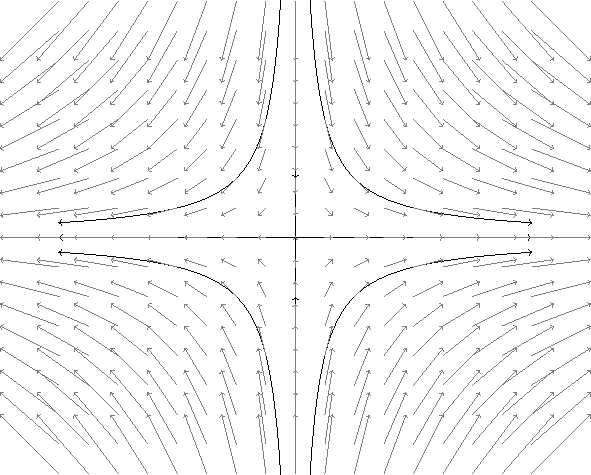
\includegraphics{figures/1-1}
        \caption{Einige Lösungen der Differentialgleichung
        zur Matrix $A = \text{diag}(1, -1)$.}%
        \label{fig:1-1}
      \end{figure}
    \item Betrachte die Matrix
      \[
          A =
          \begin{pmatrix}
            0 & -1 \\ 0 & 0
          \end{pmatrix}
      \]
      und bemerke, dass $A^2 = 0$ gilt.
      Folglich ist
      \[
        e^{tA} =
        \begin{pmatrix}
          1 & -t \\ 0 & 1
        \end{pmatrix}.
      \]
      Die Lösungskurven von $A$ 
      sind konstant auf der $x$-Achse,
      und ausserhalb sind sie parallel dazu,
      wobei ihre Geschwindigkeit mit zunehmender
      $y$-Komponente linear wächst.
    \item Die Matrix
      \[
        A = 
        \begin{pmatrix}
          0 & 0 \\ 1 & 0
        \end{pmatrix}
      \]
      liefert ein rotiertes Bild des obigen Beispiels.
    \item Die Matrix
      \[
        A =
        \begin{pmatrix}
          0 & -1 \\ 1 & 0
        \end{pmatrix}
      \]
      ist eine Drehung um den Winkel $\pi/2$.
      Die Potenzen von $A$ sind
      $A^2 = -1$, $A^3 = -A$, und $A^4 = 1$.
      Dann geht es periodisch weiter.
      Berechne
      \[
        e^{tA} =
        \begin{pmatrix}
          1 - t^2/2! + t^4/4! -  \cdots
          & -t + t^3/3! - t^5/5! + \cdots \\
          t - t^3/3! + t^5/5! - \cdots
          &
          1 - t^2/2! + t^4/4! -  \cdots
        \end{pmatrix}
        =
        \begin{pmatrix}
          \cos(t) & -\sin(t) \\
          \sin(t) & \cos(t)
        \end{pmatrix}.
      \]
      Wir haben also nun hergeleitet, dass
      die Lösungskurven dieses Vektorfelds konzentrische
      Kreise sind.
      Wir sehen auch, dass im allgemeinen
      $e^{t(A + B)} = e^{tA} \cdot e^{tB}$ nicht gilt
      (das gilt nur, wenn $AB = BA$).
  \end{enumerate}
\end{examples}

\begin{remark}
Die Matrix $e^{tA}$ lässt sich für diagonalisierbare
Matrizen $A \in \mathbb{R}^{n \times n}$ relativ einfach
berechnen. Sei $A$ eine solche Matrix, das heisst,
es existiert $P \in \mathbb{R}^{n \times n}$
mit
$\det(P) \neq 0$ und $PAP^{-1} = D = \text{diag}(\lambda_1, \dots, \lambda_n)$ 
ist diagonal.
Es gilt dann
\[
A^k = {(P^{-1}DP)}^k = P^{-1}D^k P,
\]
also folgt $e^{tA} = P^{-1}e^{tD}P$, wobei
$e^{tD} = \text{diag}(e^{t\lambda_1}, \dots, e^{t \lambda_n})$.
Dies funktioniert genau so, falls $A$ über $\mathbb{C}$ 
diagonalisierbar ist.
Für nicht diagonalisierbare $A$ wird die Jordan-Normalform
zur Berechnung von $e^{tA}$ verwendet.
Schreibe dazu $A = D + N$ für eine diagonalisierbare
Matrix $D$ und eine nilpotente Matrix $N$ mit
$DN = ND$.
\end{remark}

\section{Differentialgleichungen in einer Variable}
Sei $f \colon \mathbb{R} \to \mathbb{R}$ stetig
(aber nicht unbedingt linear).
Wir erhalten eine Differentialgleichung
für $y \colon (-T, T) \to \mathbb{R}$ 
mit $y(0) = y_0 \in \mathbb{R}$,
nämlich $\dot y = f(y(t))$.
Falls $f(y_0) = 0$, dann ist
$y(t) = y_0$ eine konstante Lösung.
Falls $f(y_0) \neq 0$, schreibe (lokal) um, dass
\[
  \dot y(t) \frac{1}{f(y(t))} = 1.
\]

\begin{lemma*}
  Mit den Voraussetzungen oben,
  sei $g \colon \mathbb{R} \to \mathbb{R}$ eine Stammfunktion
  von $1/f$, das heisst $g'(x) = 1/f(x)$.
  Dann gilt $g(y(t)) = t + c$.
\end{lemma*}

\begin{proof}
  Berechne
  \begin{align*}
    \frac{d}{dt} \, g(y(t))
    &= g'(y(t)) \cdot \frac{d}{dt} \, y(t)\\
    &= \frac{1}{f(y(t))} \dot y(t) \\
    &= 1. && \qedhere
  \end{align*}
\end{proof}

Mit etwas Glück lässt sich diese Formel nach $y(t)$ auflösen.

\begin{examples}
  \leavevmode
  \begin{enumerate}[(1)]
    \item Betrachte $f(x) = x$, das heisst, wir untersuchen
      die Differentialgleichung $\dot y(t) = y(t)$.
      Sei $y_0 > 0$ und $g(x) = \log(x)$.
      Dann sind die Voraussetzungen vom Lemma erfüllt.
      Es gilt also $\log(y(t)) = t + c$, also
      $y(t) = e^{t + c} = e^{t \cdot e^c}$.
      Mit $y(0) = e^c = y_0$ folgt $y(t) = y_0 e^t$.
    \item Sei $f(x) = x^2$, das heisst
      wir untersuchen $\dot y(t) = {(y(t))}^2$.
      Sei $y_0 \geq 0$ und
      $g(x) = -1/x$.
      Aus $-1/y(t) = t + c$ erhalten wir
      $y(t) = -1/(t + c)$.
      Mit  $y(0) = -1/c = y_0$ erhalten wir
      \[
        y(t) = \frac{1}{1/y_0 - t}.
      \]
      Im Spezialfall $y_0 = 1$ sehen wir,
      dass die Lösung $y(t) = \frac{1}{1-t}$ 
      in endlicher Zeit divergiert: es gilt
      \[
        \lim_{t \to 1} \frac{1}{1-t} = +\infty.
      \]
    \item Sei $f(x) = 2\sqrt x$. Dann ist
      $\dot y (t) = 2 \sqrt{y(t)}$.
      Wir haben $g(x) = \sqrt x$,
      also ist $\sqrt{y(t)} = t + c$.
      Wir schliessen, dass
      $y(t) = {(t + c)}^2$ eine Lösung
      ist.
      Mit $y(0) = y_0$ folgt
      $y(t) = {(t + \sqrt {y_0})}^2$.
      Im Grenzfall  $y_0 = 0$ 
      erhalten wir $y(t) = t^2$.
      Es gibt aber noch eine alternative
      Lösung zur selben Anfangsbedingung,
      nämlich $y(t) = 0$.
      Diese Differentialgleichung modelliert das
      Abflussverhalten einer Badewanne.
      Dies kann einen physikalischen Hinweis darauf geben, dass
      die Lösungen nicht eindeutig sind. Tatsächlich
      weiss man, wenn man eine leere Badewanne antrifft
      nicht, wann sie zum letzten Mal voll war.
  \end{enumerate}
\end{examples}

\begin{remarks}
   \leavevmode
   \begin{enumerate}[(i)]
   \item Die Lösugskurven brauchen nicht für alle Zeiten zu existieren.
     Im Beispiel zwei zum Beispiel galt $\lim_{t \to 1} y(t) = \infty$.
   \item Die Lösungskurven brauchen bei gegebener Anfangsbedingung nicht
     eindeutig zu sein, siehe Beispiel (3). Für die
     Eindeutigkeit ist die Lipschitz-Stetigkeit des
     Vektorfelds essentiell.
   \item Für die Existenz von Lösungen reicht
     die Stetigkeit des Vektorfelds. Diese Tatsache
     ist als ``Satz von Peano'' bekannt.
 \end{enumerate}
\end{remarks}

Seien $a_0, a_1, \dots, a_{n-1} \in \mathbb{R}$.
Wir möchten die 
\emph{lineare homogene Differentialgleichung $n$-ter Ordnung}
\[
  y^{(n)}(t) 
  + a_{n-1}y^{(n-1)}(t) 
  + \cdots 
  + a_2 y''(t) 
  + a_1 y'(t) 
  + a_0 y(t) 
  = 0
\]
mit Anfangsbedingungen $(0) = a_0, y'(0) = y_1, \dots
y^{(n-1)}(0) = y_{n-1}$.
Konkret gesucht ist eine $n$-mal differenzierbare
Lösungsfunktion $y \colon \mathbb{R} \to \mathbb{R}$ 
die diese Bedingungen erfüllt.
Unsere Methode ist es, die Differentialgleichung auf eine
lineare Differentialgleichung erster Ordnung auf $\mathbb{R}^n$ 
zurückzuführen.
Führe dazu Koordinaten
$y, y', y'', \dots, y^{(n-1)}$ auf $\mathbb{R}^n$ ein.
Schreibe
$\gamma(t) = (y(t), y'(t), \dots, y^{(n-1)}(t))$,
\[
  A =
  \begin{pmatrix}
    0 & 1 & 0 & \cdots & 0 \\
    0 & 0 & 1 & \cdots & 0 \\
      &   & \ddots & & \vdots \\
      & & &  0 & 1 \\
    -a_0 & -a_1 & -a_2 & \cdots & -a_{n-1}
  \end{pmatrix}.
\]
Dann liest sich unsere Differentialgleichung als
$\dot \gamma(t) = A \cdot \gamma(t)$.
Also ist jede lineare homogene Differentialgleichung
$n-ter$ Ordnung auf $\mathbb{R}$ äquivalent zu einer linearen
homogonen Differentialgleichung erster Ordnung auf $\mathbb{R}^n$.
Die Anfangsbedingung in unserer Formulierung lautet
$\gamma(0) = (y_0, y_1, \dots, y_{n-1})$.
Die bekannte Lösung $\gamma(t) = e^{tA} \cdot \gamma(0)$ 
liefert die gewünschte Lösung $y(t)$ durch herauslesen
der ersten Komponente von $\gamma$.

\begin{examples}
  \leavevmode
  \begin{enumerate}[(1)]
    \item Die Differentialgleichung $\ddot y(t) + y(t) = 0$ 
      ist als
      \emph{freie Schwingung}
      bekannt. In der Physik ist $\ddot y = -g/\ell \cdot y$,
      wobei $g$ die Gravitationsbeschleunigung und $l$ 
      die Länge des Pendels ist.
      Die Funktion $y$ beschreibt den Auslenkungswinkel.
      Wir betrachten den Fall $g/\ell = 1$.
      Setze $\gamma(t) = (y(t), \dot y(t))$.
      Dann ist
      \[
        \dot \gamma(t) =
        \begin{pmatrix}
          \dot y(t)
          \ddot y(t)
        \end{pmatrix}
        =
        \begin{pmatrix}
          0 & 1 \\ -1 & 0
        \end{pmatrix}
        \begin{pmatrix}
          y(t)
          \dot y(t)
        \end{pmatrix}.
      \]
      Wenn wir die Anfangbedingungen $y_0 = 0$ 
      und $y_1 = 1$ betrachten, dann ist die Lösung
      \[
        \gamma(t) =
        \begin{pmatrix}
          \cos t & \sin t \\
          -\sin t & \cos t
        \end{pmatrix}
        \begin{pmatrix}
          0 \\ 1
        \end{pmatrix}
        =
        \begin{pmatrix}
          \sin t\\
          \cos t
        \end{pmatrix}
      \]
    \item Die Differentialgleichung
      $\ddot y(t) + \dot y(t) + y(t) = 0$ 
      ist als \emph{gedämpfte Schwingung} bekannt.
      In der Physik trifft man diese Gleichung
      als $\ddot y(t) = -ky(t) - \theta \dot y (t)$ an,
      wobei $\theta$ ein Reibungsterm ist.
      Setze $\gamma(t) = (y(t), \dot y(t))$ wie oben.
      Wir erhalten die Differentialgleichung
      \[
        \dot \gamma(t) =
        \begin{pmatrix}
          0 & 1 \\
          -1 & -1
        \end{pmatrix}
        \begin{pmatrix}
          y(t) \\
          \dot y(t)
        \end{pmatrix}.
      \]
      Um die explizite Lösung $e^{tA}$ für
      \[
        A =
        \begin{pmatrix}
          0 & 1 \\
          -1 & -1
        \end{pmatrix}
      \]
      zu bestimmen,
      berechne das charakteristische
      Polynom $\chi_{A}(t) = t^2 + t + 1$
      und dessen Eigenwerte und Eigenvektoren
      $v_1$ und $v_2$
      um $A$ zu diagonalisieren.
      Vergleiche Serie 4.
  \end{enumerate}
\end{examples}




\end{document}
